% Copyright (c) 2025 Ampere Computing. All rights reserved.
% SPDX-License-Identifier: BSD-3-Clause
\documentclass{article}
\usepackage{graphicx}
\usepackage{palatino}
\usepackage{hyperref}
\usepackage{longtable}
\usepackage{fancyhdr}
\setlength{\headheight}{15.2pt}
\pagestyle{fancy}
\fancyhf{}
\fancyfoot[C]{AMPERE COMPUTING PROPRIETARY}
\fancyfoot[R]{\thepage}
\usepackage[left=1cm, right=1cm]{geometry}
\title{Connor Compiler Guide \\ Version 0.1.0\\ AMPERE COMPUTING PROPRIETARY}
\date{2025-02-14}
\begin{document}
\maketitle

\tableofcontents
\newpage
\listoftables
\newpage
\section{Change Log}
\begin{longtable}{|l|p{4in}|}
  \hline
  {\bf Version} & {\bf Changes} \\ \hline
  \hline
  \endfirsthead
  0.1 & Initial version, updated MIDR\_EL1, cleaving, FEAT\_* \\ \hline
  0.2 & Update microarchitecture overview \\ \hline
\end{longtable}
\newpage
\section{Core overview}

The Ampere core is a highly efficient, superscalar, out-of-order
microarchitecture optimized for scalability and cloud computing
workloads. It delivers predictable performance while supporting
advanced security and virtualization features, such as nested
virtualization, ground-up speculative side-channel mitigation, and
architectural support for defense against ROP/JOP-style software
attacks. \\

The core, codenamed Connor, is an ARMv9.2+ implementation, adding
support for the following extensions:
\begin{itemize}
\item FEAT\_SVE
\item FEAT\_SVE\_AES
\item FEAT\_SVE\_SHA3
\item FEAT\_SVE\_SM4
\item FEAT\_SVE\_PMULL128
\item FEAT\_SVE2
\item FEAT\_SVE\_B16B16
\item FEAT\_B16B16
\item FEAT\_FP8
\item FEAT\_FP8FMA
\item FEAT\_FPMR
\item FEAT\_FAMINMAX
\item FEAT\_LUT
\item FEAT\_WFxT
\item FEAT\_WFxT2
\item FEAT\_CSSC
\item FEAT\_PAN3
\item FEAT\_LRCPC2
\item FEAT\_AFP
\item FEAT\_Armv9\_Crypto
\end{itemize}
As in our prior core, Connor
also supports the Memory Tagging Extension and SM3/SM4 cryptography
instructions, as well as many system-level features and numerous
performance and power efficiency improvements. \\

The front end has state-of-the-art branch prediction, with a 10-cycle
recovery time from a mispredicted branch. The L1 instruction cache is
32KB; to support efficient execution of workloads with a large code
footprint, the I-cache has a high-bandwidth, low-latency connection to
the unified L2 cache. \\

Instructions coming out of the front end are decoded into internal
micro-ops (uops). The decode stage can consume up to 8 instructions
per cycle and output up to 8 uops. Some pairs of instructions can be
‘fused’ into a single uop, and the Connor core supports several new
fusion cases. \\

Uops proceed from decode through register renaming and are dispatched
into 8 independent schedulers: 4 integer, 2 FP, and 2 memory. The
integer and FP schedulers can each issue one uop per cycle, while the
memory schedulers can each issue one load and one store (address
calculation or data read) per cycle. \\

The memory unit contains a 64KB write-through L1 data cache with a
4-cycle latency (5-cycles for operations performed on the
floating-point unit), which can support two 128-bit loads and one
store update per cycle and has a full 64-byte path for data coming in
from the L2. The memory system includes advanced memory disambiguation
support to improve out-of-order execution of interleaved loads and
stores and a highly accurate L1 data prefetcher. \\

The core has a unified memory management unit (MMU) which tracks up to
12 parallel page walks for both instructions and data and contains a
2560-entry L2 TLB. The front end has a 64-entry L1 ITLB, and the
load-store unit has a 64-entry L1 DTLB. All entries in all TLBs
are ‘universal’, meaning they can store any page size, allowing
software to make best use of large pages. \\

The L2 is a 3.5MB cache which is boot-time partitionable into a
private L2 cache and portion of a larger shared L3 cache. The default
configuration is 2.5MB for a private L2 and 1MB as part of a larger
shared L3.  The L2 stores both code and data and is inclusive of the
L1 caches. The L2 can service a full 64-byte read and write every
cycle, and can track up to 64 outstanding memory requests to the
SOC. As part of the core’s focus on scalability, the L2 dynamically
tracks traffic levels on the SOC mesh, and can adjust its request rate
to minimize delays due to congestion within the SOC. \\

\begin{center}
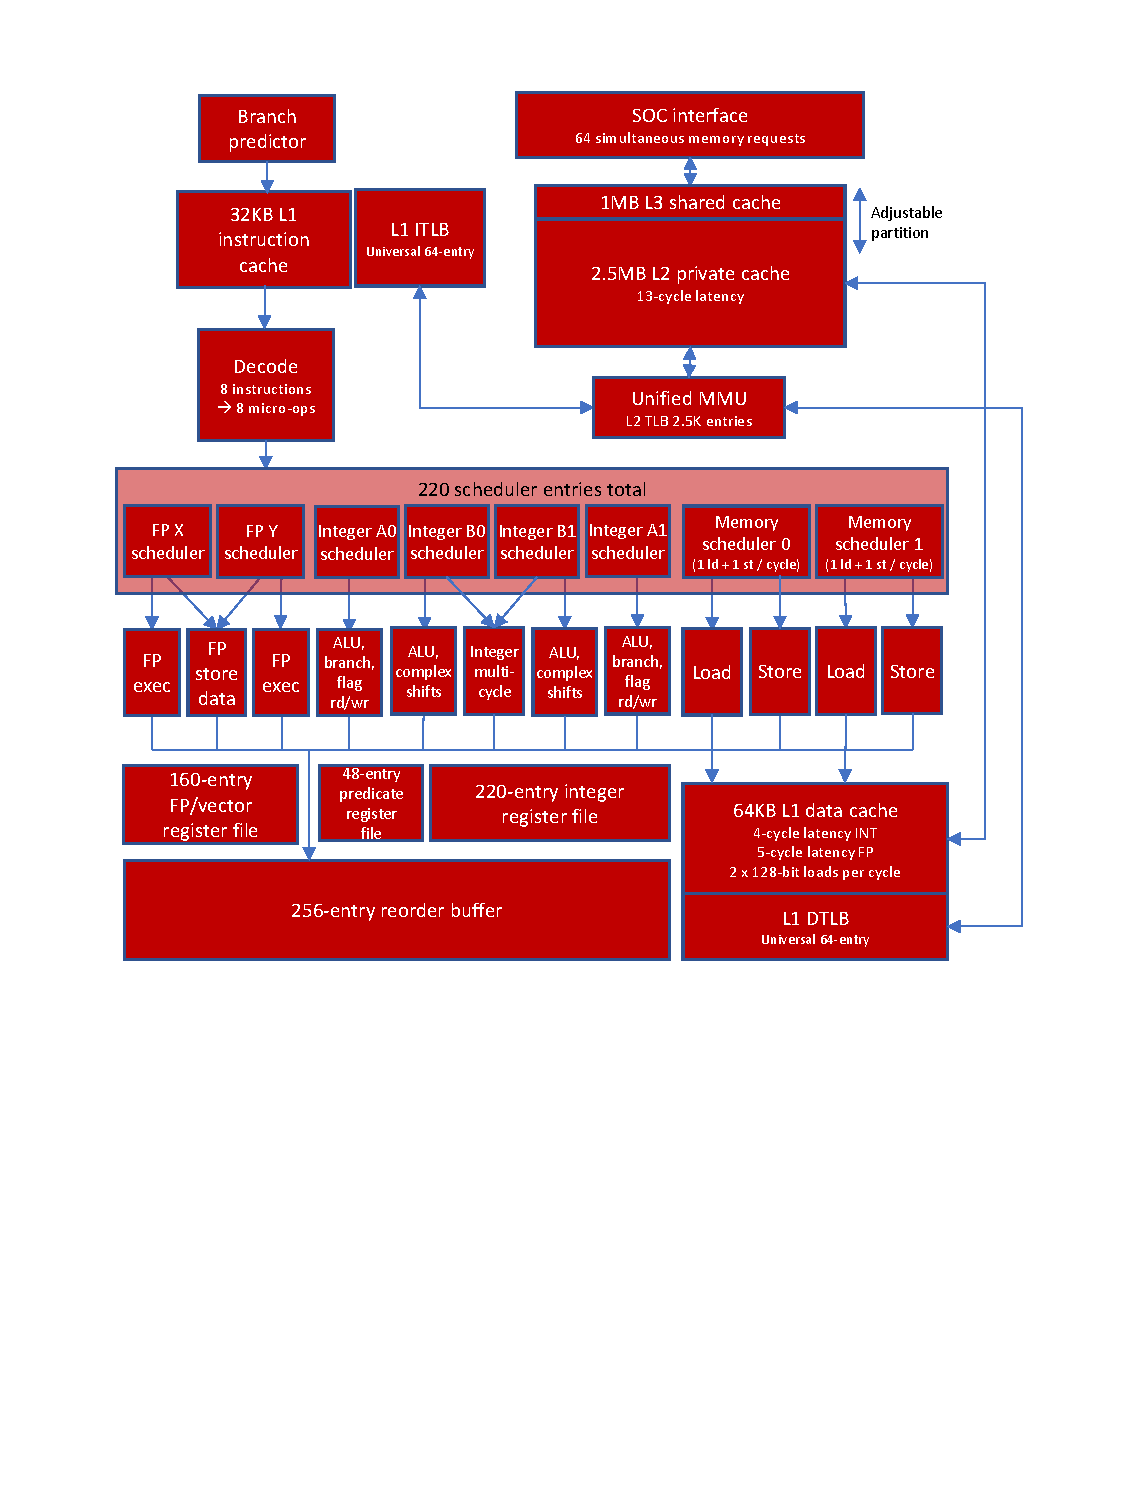
\includegraphics[height=16cm]{connor-block-diagram.pdf}
\end{center}

% MIDR_EL1 value for the Connor configuration.

\begin{figure}
\caption{Processor Identifier}
\begin{center}
  \begin{tabular}{|l|l|} \hline
    MIDR\_EL1 value &  {\tt 0xC00FAC70}  \\ \hline
    \end{tabular}
\end{center}
\end{figure}

\section{Execution pipeline overview}

Micro-ops are issued from a scheduler into one of twelve execution
pipelines. Each pipeline can generally accept and complete one uop per
cycle. The execution pipelines are shown in the following table, along
with the symbol used in the Pipelines column of the instruction
information tables below (the symbol ‘AB’ means the uop can execute on
any of the four integer pipelines, and ‘XY’ means it can execute on
either FP/vector pipe).

\begin{tabular}{|l|l|}
\hline
{\bf Pipeline} & {\bf Symbol used in tables} \\ 
\hline
2 x integer single-cycle, branch, and flags read/write & A  \\
2 x Integer single-cycle, complex shifts, flag write   & B  \\
Integer multi-cycle                                    & BS \\
2 x load                                               & L  \\
2 x store address calculation, store data              & S  \\
FP and vector operations, and flag write               & X  \\
FP and vector operations, and some crypto operations   & Y  \\
FP store data and FP to integer moves                  & Z \\
\hline 
\end{tabular}

\section{Instruction fusion}

The instruction decoder can fuse some pairs of instructions that
commonly occur together into a single uop, increasing the effective
decode and execution width of the core. Placing these instruction
pairs consecutively in memory will enable fusion and improve
performance. \\

The supported instruction fusions are:\\
\begin{longtable}{|p{2in}|p{1in}|p{1in}|p{2in}|}
\caption{Supported Fusions}
\\\hline
{\bf Description} & {\bf First instruction} & {\bf Second instruction} & {\bf Notes} \\
\hline
\endfirsthead

\hline
\multicolumn{4}{|r|}{{\tablename\ \thetable{} -- Continued from previous page}} \\
\hline
{\bf Description} & {\bf First instruction} & {\bf Second instruction} & {\bf Notes} \\
\hline
\endhead

\hline
\multicolumn{4}{|r|}{{Continued on next page}} \\
\hline
\endfoot
\hline
\endlastfoot

Flag producer + conditional branch &
SUBS (CMP), ADDS, ANDS, BICS, CCMP, CCMN &
B.cond (direct conditional branch) &
First instruction must decode to 1 uop (see tables below) – only LSL shift $<$= 4 and no sign extension \\
\hline

Arithmetic + compare and branch if zero/non-zero &
SUB, AND, EOR &
CBZ, CBNZ &
\parbox{2in}{
  \begin{enumerate}
  \item First instruction must decode to 1 uop (see tables below) – only LSL shift $<$= 4 and no sign extension
  \item Destination of the arithmetic instruction must be source of CBZ/CBNZ
\end{enumerate}} \\
\hline

ADD/SUB and set flags + Conditional set &
ADDS, SUBS &
CSET (alias of CSINC) &
Destination registers match, or the destination of the ADDS/SUBS is ZR
\\ \hline

Immediate construction &
MOVK, MOVZ &
MOVK &
\parbox{2in}{
  \begin{enumerate}
  \item Destination registers must be the same 
  \item Shift count of the two instructions must differ by 16, e.g. first shifts by 0 and second by 16
\end{enumerate}} \\
\hline

Add/subtract of 24-bit immediate &
ADD, SUB (immediate) &
ADD, SUB (immediate) &
\parbox{2in}{
  \begin{enumerate}
  \item Destination registers must be the same
  \item Destination (Rd) of the first instruction must be source (Rn) of the second
  \item One immediate must be shifted by 12 bits, and the other one not
\end{enumerate}
Example: \\
ADD X0, X1, \#1, lsl \#12 \\
ADD X0, X0, \#0xfff} \\
\hline

PC-relative address generation &
ADRP &
ADD (immediate) &
\parbox{2in}{
  \begin{enumerate}
  \item Destination registers must be the same
  \item Register source (Rn) of ADD must be the same as the destination (Rd)
  \item ADD cannot use shift/sign-extension
\end{enumerate}} \\
\hline

Compute A+B+1 or A-B-1 &
ADD, SUB (register-register) &
ADD, SUB (register, \#1) &
\parbox{2in}{
  \begin{enumerate}
  \item Destination registers must be the same
  \item First instruction must decode to 1 uop (see tables below) – only LSL shift $<$= 4 and no sign extension
  \item Destination of the first instruction must be the register source (Rn) of the second instruction
  \end{enumerate}
Example: \\
ADD X0, X1, X2\\
ADD X0, X0, \#1}
\\ \hline

Anything + NOP &
Any single-uop non-branch instruction &
NOP &
\\ \hline

Anything + B &
Any single-uop non-branch instruction &
B &
\\ \hline

AES encrypt / decrypt &
AESE,AESD &
AESMC, AESIMC &
\parbox{2in}{
  \begin{enumerate} \item Destination registers must be the same
  \item Register source (Rn) of AESMC/AESIMC must be the same as the destination (Rd)
\end{enumerate}} \\ \hline

MOVPRFX &
MOVPRFX &
supported SVE instruction &
\\ \hline
\end{longtable}

\section{SVE MOVPRFX fusion}

The core implements an optimization called movprfx-fusion for SVE
vector instructions.  When a suitable movprfx instruction precedes an
SVE vector instruction eligible for this optimization, and the
instructions align properly in the decoder, the movprfx and subsequent
SVE vector instruction are merged into one instruction. The movprfx fusion
optimization has several benefits:

\begin{enumerate}
  \item It reduces the number of instructions
    the execution engine must track and process.
  \item It converts destructive operations (that overwrite one source) into those that can have two independent sources.
  \item It can convert predicated merging operations into predicated
    zeroing operations.  Converting merging to zeroing can unlock
    increased instruction level parallelism, by breaking loop-carried
    dependences.
\end{enumerate}

The movprfx instruction has two variations: predicated and
unpredicated.  The predicated movprfx can convert operations that
default to merging with their destination register into operations
that zero elements of the destination register. The merging and
zeroing applies to elements whose governing predicate bit is
zero. Eligible unpredicated SVE instructions can only fuse with
suitable unpredicated movprfx instructions. Eligible predicated SVE
instructions can fuse with suitable predicated or unpredicated movprfx
instructions.

See the ARM Architecture Reference Manual (ARM ARM) for the detailed
rules for each instruction. At a high level, the requirements for
a movprfx instruction to be fusable with the subsequent SVE vector
instruction are:

\begin{enumerate}
  \item For predicated movprfx fusion, the movprfx predicate register name
    must match the subsequent instruction's predicate register name.
  \item For predicated movprfx fusion, the element size of the movprfx
    instruction must be the larger of the destination element size and
    the first source of the subsequent instruction.
  \item The destination register of the movprfx instruction must be
    the same as the destination register in the subsequent
    instruction.
  \item The destination register must not also be one of the sources
    of the second instruction.
\end{enumerate}

See Section~\ref{sec-movprfx-table} for a detailed list of SVE vector
instructions that are able to fuse with a suitable immediately prior
movprfx instruction.

\section{Instruction cleaving}

Cleaving packs two uops into a single decode lane when they meet
various restrictions. Cleaved uops will decode, dispatch and commit
together, potentially greatly increasing the execution throughput of
the core. As a result of cleaving, the decoder output can represent up
to 8 uops. Cleaved uops require only one reorder buffer (ROB) entry,
making the ROB appear larger when cleaving can be employed.

A pair of consecutive instructions may be able to cleave if:
\begin{itemize}
\item They both decode to a single uop
\item They do not read or write floating-point or vector registers
\item Together they do not write more than two destination registers
\item Together they do not have more than three register sources
\item They do not both write arithmetic flags
\item The first instruction is not a branch which could mispredict
\item The second instruction cannot fault, e.g. a load or store
\end{itemize}

\section{Instruction alignment}

Branch density and branch target alignment can affect performance. For
best performance, consider the following guidelines:
\begin{itemize}
\item Avoid placing more than four branch instructions in an aligned
  32-byte memory region.
\item Align branch targets to 32-byte boundaries to ensure that the
  instruction fetch unit can issue the maximum number of instructions
  after the branch.
\item Loops should span as few aligned 32-byte memory regions as
  possible; in particular, small loops of up to 8 instructions should
  reside within a single 32-byte region if possible.
\end{itemize}

For regular loops which perform the same control flow repeatedly,
Domino can achieve significant frontend power savings by entering a
special "loop mode". For loops with very few instructions (i.e. 3),
this mode can additionally increase frontend throughput in some
cases. Loop mode works best when loops have many iterations --- it is
helpful to structure code such that inner loops have many iterations
before exiting to the outer loop. In order to be a candidate for loop
mode, a loop's iterations must contain 8 or fewer total cacheline
transitions and/or taken branches, 32 or fewer instructions, and at
least one direct branch which is consistently taken each
iteration. When entering loop mode, loops with very short iterations will be unrolled in hardware (in multiples of the original loop iteration length) until there are at least 8 instructions per group of unrolled iterations. When unrolling, the above limitations apply to the full group of unrolled iterations: there must be 8 or fewer total cacheline transitions and taken branches. (For example, a 7-instruction loop containing 5 cacheline transitions/taken branches per iteration will not benefit from loop mode.)

\section{Data alignment}

The ARM architecture allows most load and store instructions to have
arbitrarily aligned addresses. As long as the data for a single load
or store operation all falls within a 64-byte cache line, the core can
handle any alignment without penalty. Loads which cross a 64-byte
boundary have longer latency, and stores which cross a 64-byte
boundary see lower bandwidth when writing the cache. \\

LDP (load-pair) and STP (store-pair) instructions of up to 16 bytes
are executed as a single memory access, so for best performance the
total range of memory being accessed by the instruction should not
split cache lines. This is in contrast to some older cores which may
have implemented LDP/STP as two separate loads or stores, so that
alignment to half of the total memory size would be sufficient to
avoid line splits. \\

A load which gets some (but not all) of its data from a recently
executed older store may also have longer latency. This can happen if
loads and stores with different sizes and/or alignments are
intermixed. \\

Two stores of 8 bytes or less to the same cache line, without any
intervening stores, may see increased write bandwidth to the cache.

\section{Optimizing memory copy}

For maximum throughput of memory copy and similar loops, vector loads
and stores are preferred over load-pair/store-pair because they can
transfer 16 bytes of data using a single register, reducing the
pressure on register renaming. Stores should be aligned on a 16-byte
boundary whenever possible. If the source and destination cannot both
be 16-byte aligned, it is better to align the destination. The
following example shows a recommended sequence for a long memory copy:
\begin{verbatim}
loop_start:
ldr   q0, [x0, #16]
ldr   q1, [x0, #32]
ldr   q2, [x0, #48]
ldr   q3, [x0, #64]!
str   q0, [x1, #16]
str   q1, [x1, #32]
str   q2, [x1, #48]
str   q3, [x1, #64]!
subs  x2, x2, #64
b.ne  loop_start
\end{verbatim}

\section{FP/vector bypassing}

Floating point and vector execution is divided into different units,
which contain operations which are commonly used together. The
bypassing logic is optimized to give the best latency for operations
within the same unit. \\

The latencies in the instruction tables assume that the result is
consumed within the same unit. If the result is consumed in a
different FP unit, the producing instruction may have a longer
effective latency. In the instruction tables below, the FP unit column
shows which unit an instruction executes in; if two units are shown,
then the instruction consumes its input registers in the first unit,
and produces its output register in the second unit. \\

The units and the extra latency to bypass between units are shown in this table: \\
\begin{tabular}{|l|l|p{2in}|}
\hline
{\bf Unit name} & {\bf Function}  & {\bf Extra latency if result is consumed in a different unit} \\ \hline
MA & FP arithmetic and multiplication, single/double precision & 2 or 3 (6 cycles total)  \\
HP & FP arithmetic and multiplication, half precision & 2  \\
DV & FP division and square root & 0  \\
BY & Simple logical and shuffle operations & 0  \\
BU & Bfloat16 arithmetic & 5  \\
SI & ASIMD integer arithmetic and logical & 1 or 2  \\
MU & ASIMD integer multiplication & 3 to SI, 4 to others  \\
CU & Cryptography operations & 1 or 2  \\ \hline
\end{tabular}
\\

Instructions which cross elements from one lane to another, such as
 by-element, lengthening, and pairwise instructions, may incur extra
 latency depending on the producer of the data sources and which
 operand of the instruction is consuming the data. This lane-crossing
 latency is 1 cycle in the SI and MU units, 2 cycles in the HP unit,
 and 2 or 3 cycles in the MA unit. A single instruction will not have
 both cross-unit and cross-element extra latency. \\

All FP units other than DV are fully pipelined and can complete one
 operation per cycle, and most operations are supported on both FP
 execution pipelines for maximum throughput. \\

 \subsection{Late accumulate optimization}

 For BU operations and MU operations that have accumulator operands
 (except for the byte-width MLA and MLS MU instructions), the
 accumulator operand is permitted to arrive 3 cycles after the
 operation issues.  This optimization has the effect of shortening the
 observed latency when performing a sequence of similar operations
 that support the late accumulate optimization.  When the late
 accumulate optimization is not used, say because the program is not
 performing a sequence of late-accumulate operations, MU operations
 are nominally 6 or 7 cycles. BU operations are nominally 7 cycles.

\newpage
\section{Instruction information}
\newpage
\begin{longtable}{|p{1in}|p{1in}|l|l|l|p{1in}|l|p{1in}|}
\caption{Branch Instructions} \\
\hline
Group & Instructions & Latency & Throughput & Uop count & Pipelines & FP unit & Notes\\
\hline
\endfirsthead
\hline
\multicolumn{8}{|r|}{{\tablename\ \thetable{} -- Continued from previous page}} \\
\hline
Group & Instructions & Latency & Throughput & Uop count & Pipelines & FP unit & Notes\\
\hline
\endhead
\hline
\multicolumn{8}{|r|}{{Continued on next page}} \\
\hline
\endfoot
\hline
\endlastfoot
Branch & B.$<$cond$>$, BL, BR, CBNZ, CBZ, RET, TBNZ, TBZ & 1 & 2 & 1 & A &  & \\
\hline
Indirect call & BLR & 1 & 1 & 2 & A A &  & \\
\hline
\end{longtable}
\newpage
\begin{longtable}{|p{1in}|p{1in}|l|l|l|p{1in}|l|p{1in}|}
\caption{Common Short Sequence Compression (FEAT\_CSSC)} \\
\hline
Group & Instructions & Latency & Throughput & Uop count & Pipelines & FP unit & Notes\\
\hline
\endfirsthead
\hline
\multicolumn{8}{|r|}{{\tablename\ \thetable{} -- Continued from previous page}} \\
\hline
Group & Instructions & Latency & Throughput & Uop count & Pipelines & FP unit & Notes\\
\hline
\endhead
\hline
\multicolumn{8}{|r|}{{Continued on next page}} \\
\hline
\endfoot
\hline
\endlastfoot
Absolute value & ABS & 1 & 4 & 1 & AB &  & \\
\hline
Population Count & CNT & 3 & 1 & 1 & BS &  & \\
\hline
Signed Max/ Min & SMAX, SMIN & 1 & 2 & 2 & AB A &  & \\
\hline
Trailing Zeros Count & CTZ & 1 & 2 & 1 & B &  & \\
\hline
Unsigned Max/ Min & UMAX, UMIN & 1 & 2 & 2 & AB A &  & \\
\hline
\end{longtable}
\newpage
\begin{longtable}{|p{1in}|p{1in}|l|l|l|p{1in}|l|p{1in}|}
\caption{Integer Miscellaneous Instructions} \\
\hline
Group & Instructions & Latency & Throughput & Uop count & Pipelines & FP unit & Notes\\
\hline
\endfirsthead
\hline
\multicolumn{8}{|r|}{{\tablename\ \thetable{} -- Continued from previous page}} \\
\hline
Group & Instructions & Latency & Throughput & Uop count & Pipelines & FP unit & Notes\\
\hline
\endhead
\hline
\multicolumn{8}{|r|}{{Continued on next page}} \\
\hline
\endfoot
\hline
\endlastfoot
Address generation & ADR, ADRP & 1 & 2 & 1 & A &  & \\
\hline
Bitfield extract & EXTR & 1 & 2 & 1 & B &  & \\
\hline
Bitfield move & BFM, SBFM, UBFM & 1 & 2 & 1 & B &  & \\
\hline
CRC & CRC32B, CRC32CB, CRC32CH, CRC32CW, CRC32CX, CRC32H, CRC32W, CRC32X & 3 & 1 & 1 & BS &  & \\
\hline
Count leading & CLS, CLZ & 1 & 2 & 1 & B &  & \\
\hline
Flag write & SETF16, SETF8 & 1 & 2 & 1 & A &  & \\
\hline
Move immediate & MOVK, MOVN, MOVZ & 1 & 4 & 1 & AB &  & \\
\hline
Reverse bits/ bytes & RBIT, REV, REV16, REV32 & 1 & 2 & 1 & B &  & \\
\hline
Table lookup with 2-bit indices & LUTI2 & 2 & 2 & 1 & XY & SI & \\
\hline
Table lookup with 4-bit indices & LUTI4 & 2 & 2 & 1 & XY & SI & \\
\hline
Variable shift & ASRV, LSLV, LSRV, RORV & 1 & 2 & 1 & B &  & \\
\hline
\end{longtable}
\newpage
\begin{longtable}{|p{1in}|p{1in}|l|l|l|p{1in}|l|p{1in}|}
\caption{Integer arithmetic and logical Instructions} \\
\hline
Group & Instructions & Latency & Throughput & Uop count & Pipelines & FP unit & Notes\\
\hline
\endfirsthead
\hline
\multicolumn{8}{|r|}{{\tablename\ \thetable{} -- Continued from previous page}} \\
\hline
Group & Instructions & Latency & Throughput & Uop count & Pipelines & FP unit & Notes\\
\hline
\endhead
\hline
\multicolumn{8}{|r|}{{Continued on next page}} \\
\hline
\endfoot
\hline
\endlastfoot
Arithmetic, reading flags & ADC, SBC & 1 & 2 & 1 & A &  & \\
\hline
Arithmetic/ logical, LSL shift $<$= 4 & ADD, AND, BIC, EON, EOR, ORN, ORR, SUB & 1 & 4 & 1 & AB &  & \\
\hline
Arithmetic/ logical, LSR/ ASR/ ROR shift or LSL shift $>$ 4 & ADD, AND, BIC, EON, EOR, ORN, ORR, SUB & 2 & 2 & 2 & B AB &  & \\
\hline
Arithmetic/ logical, LSR/ ASR/ ROR shift or LSL shift $>$ 4, setting flags & ADDS, ANDS, BICS, SUBS & 2 & 2 & 2 & B AB &  & \\
\hline
Arithmetic/ logical, extended register & ADD, BIC, EON, ORN, SUB & 2 & 2 & 2 & AB AB &  & \\
\hline
Arithmetic/ logical, reading and setting flags & ADCS, RMIF, SBCS & 1 & 2 & 1 & A &  & \\
\hline
Arithmetic/ logical, setting flags & ADDS, ANDS, BICS, SUBS & 1 & 4 & 1 & AB &  & \\
\hline
Arithmetic/ logical, setting flags, extended register & ADDS, BICS, SUBS & 2 & 2 & 2 & AB AB &  & \\
\hline
Conditional compare & CCMN, CCMP & 1 & 2 & 1 & A &  & \\
\hline
Conditional select & CSEL, CSINC, CSINV, CSNEG & 1 & 2 & 1 & A &  & \\
\hline
Divide, W-form & SDIV, UDIV & 21 & 2/ 21 & 2 & BS X & DV & Variable latency\\
\hline
Divide, X-form & SDIV, UDIV & 30 & 2/ 30 & 3 & BS BS X & DV & Variable latency\\
\hline
Multiply & MADD, SMADDL, SMULH, UMADDL, UMULH & 3 & 1 & 1 & BS &  & \\
\hline
Multiply-add/ subtract & MADD, MSUB, SMADDL, SMSUBL, UMADDL, UMSUBL & 4 & 1 & 2 & BS AB &  & \\
\hline
\end{longtable}
\newpage
\begin{longtable}{|p{1in}|p{1in}|l|l|l|p{1in}|l|p{1in}|}
\caption{Integer load Instructions} \\
\hline
Group & Instructions & Latency & Throughput & Uop count & Pipelines & FP unit & Notes\\
\hline
\endfirsthead
\hline
\multicolumn{8}{|r|}{{\tablename\ \thetable{} -- Continued from previous page}} \\
\hline
Group & Instructions & Latency & Throughput & Uop count & Pipelines & FP unit & Notes\\
\hline
\endhead
\hline
\multicolumn{8}{|r|}{{Continued on next page}} \\
\hline
\endfoot
\hline
\endlastfoot
Load pair & LDNP, LDP, LDPSW & 3 & 2 & 1 & L &  & \\
\hline
Load register & LDR, LDRB, LDRH, LDRSB, LDRSH, LDRSW, LDTR, LDTRB, LDTRH, LDTRSB, LDTRSH, LDTRSW, LDUR, LDURB, LDURH, LDURSB, LDURSH, LDURSW & 3 & 2 & 1 & L &  & \\
\hline
Prefetch & PRFM, PRFUM & 1 & 2 & 1 & L &  & \\
\hline
\end{longtable}
\newpage
\begin{longtable}{|p{1in}|p{1in}|l|l|l|p{1in}|l|p{1in}|}
\caption{Integer store Instructions} \\
\hline
Group & Instructions & Latency & Throughput & Uop count & Pipelines & FP unit & Notes\\
\hline
\endfirsthead
\hline
\multicolumn{8}{|r|}{{\tablename\ \thetable{} -- Continued from previous page}} \\
\hline
Group & Instructions & Latency & Throughput & Uop count & Pipelines & FP unit & Notes\\
\hline
\endhead
\hline
\multicolumn{8}{|r|}{{Continued on next page}} \\
\hline
\endfoot
\hline
\endlastfoot
Store pair with non-temporal hint & STNP & 1 & 2 & 1 & S &  & \\
\hline
Store pair, D-form & STP & 1 & 2 & 1 & S &  & \\
\hline
Store pair, W-form & STP & 2 & 2 & 2 & B S &  & \\
\hline
Store pair, pre/ post-index, W-form & STP & 2 & 2 & 3 & B S AB &  & \\
\hline
Store register, immediate offset & STR, STRB, STRH, STTR, STTRB, STTRH, STUR, STURB, STURH & 1 & 2 & 1 & S &  & \\
\hline
Store register, register offset & STR, STRB, STRH & 1 & 2 & 1 & S &  & \\
\hline
\end{longtable}
\newpage
\begin{longtable}{|p{1in}|p{1in}|l|l|l|p{1in}|l|p{1in}|}
\caption{Memory tagging} \\
\hline
Group & Instructions & Latency & Throughput & Uop count & Pipelines & FP unit & Notes\\
\hline
\endfirsthead
\hline
\multicolumn{8}{|r|}{{\tablename\ \thetable{} -- Continued from previous page}} \\
\hline
Group & Instructions & Latency & Throughput & Uop count & Pipelines & FP unit & Notes\\
\hline
\endhead
\hline
\multicolumn{8}{|r|}{{Continued on next page}} \\
\hline
\endfoot
\hline
\endlastfoot
Insert pseudo-random tag & IRG & 4 & 1 & 2 & BS B &  & \\
\hline
Load tag & LDG & 4 & 2 & 2 & L B &  & \\
\hline
Store tag & STG & 1 & 2 & 1 & S &  & \\
\hline
Store tag and pair of registers & STGP & 1 & 2 & 1 & S &  & \\
\hline
Store tag and zero data & STZG & 1 & 2 & 1 & S &  & \\
\hline
Store two tags & ST2G & 1 & 1 & 2 & S S &  & \\
\hline
Store two tags and zero data & STZ2G & 1 & 1 & 2 & S S &  & \\
\hline
Subtract pointer & SUBP & 1 & 4 & 1 & AB &  & \\
\hline
Subtract pointer, setting flags & SUBPS & 1 & 4 & 1 & AB &  & \\
\hline
Tag mask insert & GMI & 1 & 4 & 1 & AB &  & \\
\hline
Tagged pointer arithmetic & ADDG, SUBG & 1 & 2 & 1 & B &  & \\
\hline
\end{longtable}
\newpage
\begin{longtable}{|p{1in}|p{1in}|l|l|l|p{1in}|l|p{1in}|}
\caption{Pointer authentication} \\
\hline
Group & Instructions & Latency & Throughput & Uop count & Pipelines & FP unit & Notes\\
\hline
\endfirsthead
\hline
\multicolumn{8}{|r|}{{\tablename\ \thetable{} -- Continued from previous page}} \\
\hline
Group & Instructions & Latency & Throughput & Uop count & Pipelines & FP unit & Notes\\
\hline
\endhead
\hline
\multicolumn{8}{|r|}{{Continued on next page}} \\
\hline
\endfoot
\hline
\endlastfoot
Authenticate address & AUTDA, AUTDB, AUTDZA, AUTDZB, AUTIA, AUTIB, AUTIZA, AUTIZB & 5 & 1 & 1 & BS &  & \\
\hline
Branch with authentication & BRAA, BRAAZ, BRAB, BRABZ, RETAA, RETAB & 6 & 1 & 2 & BS A &  & When associated key is disabled by SCTLR\_ELx, latency is reduced by 5 cycles\\
\hline
Call with authentication & BLR & 2 & 1 & 3 & AB A A &  & \\
\hline
Call with authentication & BLRAA, BLRAAZ, BLRAB, BLRABZ & 6 & 1 & 3 & BS A A &  & When associated key is disabled by SCTLR\_ELx, latency is reduced by 5 cycles\\
\hline
Generate authentication code & PACDA, PACDB, PACDZA, PACDZB, PACGA, PACIA, PACIB, PACIZA, PACIZB & 5 & 1 & 1 & BS &  & \\
\hline
Load register with authentication & LDRAA, LDRAB & 8 & 1 & 2 & BS L &  & When associated key is disabled by SCTLR\_ELx, latency is reduced by 5 cycles\\
\hline
Load register with authentication, pre-increment & LDRAA, LDRAB & 8 & 1 & 3 & BS L AB &  & When associated key is disabled by SCTLR\_ELx, latency is reduced by 5 cycles\\
\hline
Remove authentication code & XPACD, XPACI & 1 & 2 & 1 & B &  & \\
\hline
\end{longtable}
\newpage
\begin{longtable}{|p{1in}|p{1in}|l|l|l|p{1in}|l|p{1in}|}
\caption{ASIMD Bfloat16 Instructions} \\
\hline
Group & Instructions & Latency & Throughput & Uop count & Pipelines & FP unit & Notes\\
\hline
\endfirsthead
\hline
\multicolumn{8}{|r|}{{\tablename\ \thetable{} -- Continued from previous page}} \\
\hline
Group & Instructions & Latency & Throughput & Uop count & Pipelines & FP unit & Notes\\
\hline
\endhead
\hline
\multicolumn{8}{|r|}{{Continued on next page}} \\
\hline
\endfoot
\hline
\endlastfoot
Bfloat16 conversion & BF1CVTL{{2}}, BF2CVTL{{2}} & 3 & 2 & 1 & XY & HP & \\
\hline
\end{longtable}
\newpage
\begin{longtable}{|p{1in}|p{1in}|l|l|l|p{1in}|l|p{1in}|}
\caption{ASIMD Cryptography Instructions} \\
\hline
Group & Instructions & Latency & Throughput & Uop count & Pipelines & FP unit & Notes\\
\hline
\endfirsthead
\hline
\multicolumn{8}{|r|}{{\tablename\ \thetable{} -- Continued from previous page}} \\
\hline
Group & Instructions & Latency & Throughput & Uop count & Pipelines & FP unit & Notes\\
\hline
\endhead
\hline
\multicolumn{8}{|r|}{{Continued on next page}} \\
\hline
\endfoot
\hline
\endlastfoot
AES encryption/ decryption & AESD, AESE, AESIMC, AESMC & 2 & 2 & 1 & XY & CU & Fused pairs have 2-cycle latency\\
\hline
Polynomial multiplication & PMUL, PMULL{{2}} & 2 & 2 & 1 & XY & CU & \\
\hline
SHA-256 hash & SHA256H, SHA256H2 & 4 & 1 & 1 & X & CU & \\
\hline
SHA-256 schedule update & SHA256SU0, SHA256SU1 & 2 & 1 & 1 & Y & CU & \\
\hline
SHA-3 Instructions & BCAX, EOR3, RAX1, XAR & 2 & 2 & 1 & XY & CU & \\
\hline
SHA-512 hash & SHA512H, SHA512H2 & 4 & 1 & 1 & X & CU & \\
\hline
SHA-512 schedule update & SHA512SU0, SHA512SU1 & 2 & 1 & 1 & Y & CU & \\
\hline
SHA1 choose/ majority/ parity & SHA1C, SHA1M, SHA1P & 4 & 1 & 1 & X & CU & \\
\hline
SHA1 hash/ schedule update & SHA1H, SHA1SU0, SHA1SU1 & 2 & 1 & 1 & Y & CU & \\
\hline
SM3 hash & SM3PARTW1, SM3PARTW2, SM3SS1, SM3TT1A, SM3TT1B, SM3TT2A, SM3TT2B & 2 & 2 & 1 & XY & CU & \\
\hline
SM4 encryption & SM4E, SM4EKEY & 4 & 1 & 1 & X & CU & \\
\hline
\end{longtable}
\newpage
\begin{longtable}{|p{1in}|p{1in}|l|l|l|p{1in}|l|p{1in}|}
\caption{ASIMD FP Miscellaneous Instructions} \\
\hline
Group & Instructions & Latency & Throughput & Uop count & Pipelines & FP unit & Notes\\
\hline
\endfirsthead
\hline
\multicolumn{8}{|r|}{{\tablename\ \thetable{} -- Continued from previous page}} \\
\hline
Group & Instructions & Latency & Throughput & Uop count & Pipelines & FP unit & Notes\\
\hline
\endhead
\hline
\multicolumn{8}{|r|}{{Continued on next page}} \\
\hline
\endfoot
\hline
\endlastfoot
Convert ASIMD FP to integer in GPR & FCVTAS, FCVTAU, FCVTMS, FCVTMU, FCVTNS, FCVTNU, FCVTPS, FCVTPU, FCVTZS, FCVTZU & 7 & 1 & 2 & XY Z & MA & \\
\hline
Convert ASIMD FP to integer in GPR, fixed-point round to zero & FCVTZS, FCVTZU & 10 & 1 & 3 & XY XY Z & MA & \\
\hline
Convert ASIMD FP32 to ASIMD FP8 & FCVTN{{2}} & 8 & 1 & 2 & XY XY & MA,BY & \\
\hline
Convert precision from half & FCVT & 3 & 2 & 1 & XY & MA & \\
\hline
Convert precision from single/ double & FCVT & 3 & 2 & 1 & XY & MA & \\
\hline
Convert to higher precision long & FCVTL{{2}} & 3 & 2 & 1 & XY & MA & \\
\hline
Convert to lower precision from double & FCVTXN{{2}} & 8 & 1 & 2 & XY XY & MA,BY & \\
\hline
Convert to lower precision from double, rounding to odd & FCVTXN & 3 & 2 & 1 & XY & MA & \\
\hline
Convert to lower precision from single/ double & FCVTN{{2}} & 8 & 1 & 2 & XY XY & MA,BY & \\
\hline
Javascript convert ASIMD FP to integer & FJCVTZS & 7 & 1 & 2 & X Z & MA & \\
\hline
Move GPR to vector register & FMOV & 5 & 1 & 1 & BS &  & \\
\hline
Move from GPR to upper element & FMOV & 7 & 1 & 2 & BS XY & BY & \\
\hline
Move register/ immediate & FMOV & 2 & 2 & 1 & XY & BY & \\
\hline
Move upper element to GPR & FMOV & 5 & 1 & 1 & X & BY & \\
\hline
Move vector register to GPR & FMOV & 3 & 1 & 1 & Z &  & \\
\hline
\end{longtable}
\newpage
\begin{longtable}{|p{1in}|p{1in}|l|l|l|p{1in}|l|p{1in}|}
\caption{ASIMD FP and vector load Instructions} \\
\hline
Group & Instructions & Latency & Throughput & Uop count & Pipelines & FP unit & Notes\\
\hline
\endfirsthead
\hline
\multicolumn{8}{|r|}{{\tablename\ \thetable{} -- Continued from previous page}} \\
\hline
Group & Instructions & Latency & Throughput & Uop count & Pipelines & FP unit & Notes\\
\hline
\endhead
\hline
\multicolumn{8}{|r|}{{Continued on next page}} \\
\hline
\endfoot
\hline
\endlastfoot
Load 1-element structure to one/ all lanes & LD1, LD1R & 6 & 2 & 2 & L XY & BY & \\
\hline
Load 1-element structure to one/ all lanes, 1D size & LD1R & 4 & 2 & 1 & L &  & \\
\hline
Load 1-element structures to 1 register & LD1 & 4 & 2 & 1 & L &  & \\
\hline
Load 1-element structures to 2 registers & LD1 & 4 & 1 & 2 & L L &  & \\
\hline
Load 1-element structures to 3 registers & LD1 & 5 & 2/ 3 & 3 & L L L &  & \\
\hline
Load 1-element structures to 4 registers & LD1 & 5 & 1/ 2 & 4 & L L L L &  & \\
\hline
Load 2-element structure to all lanes of 2 registers, 1D size & LD2R & 4 & 1 & 2 & L L &  & \\
\hline
Load 2-element structure to all lanes of 2 registers, other sizes & LD2R & 6 & 1 & 4 & L L XY XY & BY & \\
\hline
Load 2-element structure to one lane of 2 registers & LD2 & 6 & 1 & 4 & L L XY XY & BY & \\
\hline
Load 2-element structures to 2 registers, 16B/ 8H/ 4S/ 2D size & LD2 & 6 & 1 & 4 & L L XY XY & BY & \\
\hline
Load 2-element structures to 2 registers, 8B/ 4H/ 2S size & LD2 & 8 & 2/ 3 & 5 & L L XY XY XY & BY & \\
\hline
Load 3-element structure to all lanes of 3 registers, 1D size & LD3R & 5 & 2/ 3 & 3 & L L L &  & \\
\hline
Load 3-element structure to all lanes of 3 registers, other sizes & LD3R & 7 & 2/ 3 & 6 & L L L XY XY XY & BY & \\
\hline
Load 3-element structure to one lane of 3 registers & LD3 & 7 & 2/ 3 & 6 & L L L XY XY XY & BY & \\
\hline
Load 3-element structures to 3 registers, 16B/ 8H/ 4S sizes & LD3 & 8 & 2/ 3 & 6 & L L L XY XY XY & BY & \\
\hline
Load 3-element structures to 3 registers, 2D size & LD3 & 7 & 2/ 3 & 6 & L L L XY XY XY & BY & \\
\hline
Load 3-element structures to 3 registers, 8B/ 4H/ 2S sizes & LD3 & 9 & 1/ 2 & 7 & L L L XY XY XY XY & BY & \\
\hline
Load 4-element structure to all lanes of 4 registers, 1D size & LD4R & 5 & 1/ 2 & 4 & L L L L &  & \\
\hline
Load 4-element structure to all lanes of 4 registers, other sizes & LD4R & 7 & 1/ 2 & 8 & L L L L XY XY XY XY & BY & \\
\hline
Load 4-element structure to one lane of 4 registers & LD4 & 7 & 1/ 2 & 8 & L L L L XY XY XY XY & BY & \\
\hline
Load 4-element structures to 4 registers, 2D size & LD4 & 8 & 1/ 2 & 8 & L L L L XY XY XY XY & BY & \\
\hline
Load 4-element structures to 4 registers, 2S size & LD4 & 11 & 1/ 4 & 12 & L L L L XY XY XY XY XY XY XY XY & BY & \\
\hline
Load 4-element structures to 4 registers, other sizes & LD4 & 10 & 1/ 4 & 12 & L L XY XY L L XY XY XY XY XY XY & BY & \\
\hline
Load pair, Q-form & LDNP, LDP & 4 & 1 & 2 & L L &  & \\
\hline
Load pair, S/ D-form & LDNP, LDP & 5 & 1 & 2 & L BS &  & \\
\hline
Load register & LDR, LDUR & 4 & 2 & 1 & L &  & \\
\hline
\end{longtable}
\newpage
\begin{longtable}{|p{1in}|p{1in}|l|l|l|p{1in}|l|p{1in}|}
\caption{ASIMD FP and vector store Instructions} \\
\hline
Group & Instructions & Latency & Throughput & Uop count & Pipelines & FP unit & Notes\\
\hline
\endfirsthead
\hline
\multicolumn{8}{|r|}{{\tablename\ \thetable{} -- Continued from previous page}} \\
\hline
Group & Instructions & Latency & Throughput & Uop count & Pipelines & FP unit & Notes\\
\hline
\endhead
\hline
\multicolumn{8}{|r|}{{Continued on next page}} \\
\hline
\endfoot
\hline
\endlastfoot
Store 1-element structure from one lane of 1 register & ST1 & 4 & 1 & 3 & XY S Z & BY & \\
\hline
Store 1-element structures from 1 register & ST1 & 2 & 1 & 2 & S Z &  & \\
\hline
Store 1-element structures from 2 registers & ST1 & 3 & 1/ 2 & 4 & S Z S Z &  & \\
\hline
Store 1-element structures from 3 registers & ST1 & 4 & 1/ 3 & 6 & S Z S Z S Z &  & \\
\hline
Store 1-element structures from 4 registers & ST1 & 5 & 1/ 4 & 8 & S Z S Z S Z S Z &  & \\
\hline
Store 2-element structure from one lane of 2 registers & ST2 & 5 & 1/ 2 & 6 & XY XY S Z S Z & BY & \\
\hline
Store 2-element structures from 2 registers, 16B/ 8H/ 4S/ 2D sizes & ST2 & 5 & 1/ 2 & 6 & XY XY S Z S Z & BY & \\
\hline
Store 2-element structures from 2 registers, 8B/ 4H/ 2S sizes & ST2 & 6 & 1/ 2 & 6 & XY XY S Z S Z & BY & \\
\hline
Store 3-element structure from one lane of 3 registers & ST3 & 6 & 1/ 3 & 9 & XY XY XY S Z S Z S Z & BY & \\
\hline
Store 3-element structures from 3 registers & ST3 & 6 & 1/ 3 & 9 & XY XY XY S Z S Z S Z & BY & \\
\hline
Store 4-element structure from one lane of 4 registers & ST4 & 7 & 1/ 4 & 12 & XY XY XY XY S Z S Z S Z S Z & BY & \\
\hline
Store 4-element structures from 4 registers, 16B/ 8H/ 4S sizes & ST4 & 7 & 1/ 4 & 12 & XY XY S X S X XY XY S X S X & BY & \\
\hline
Store 4-element structures from 4 registers, 2D sizes & ST4 & 7 & 1/ 4 & 12 & XY XY XY XY S Z S Z S Z S Z & BY & \\
\hline
Store 4-element structures from 4 registers, 8B/ 4H/ 2S sizes & ST4 & 9 & 1/ 4 & 14 & XY XY XY XY XY XY S Z S Z S Z S Z & BY & \\
\hline
Store pair, Q-form & STNP, STP & 3 & 1/ 2 & 4 & S Z S Z &  & \\
\hline
Store pair, S/ D-form & STNP, STP & 3 & 1/ 2 & 3 & S Z Z &  & \\
\hline
Store register & STR, STUR & 2 & 1 & 2 & S Z &  & \\
\hline
\end{longtable}
\newpage
\begin{longtable}{|p{1in}|p{1in}|l|l|l|p{1in}|l|p{1in}|}
\caption{ASIMD FP data processing} \\
\hline
Group & Instructions & Latency & Throughput & Uop count & Pipelines & FP unit & Notes\\
\hline
\endfirsthead
\hline
\multicolumn{8}{|r|}{{\tablename\ \thetable{} -- Continued from previous page}} \\
\hline
Group & Instructions & Latency & Throughput & Uop count & Pipelines & FP unit & Notes\\
\hline
\endhead
\hline
\multicolumn{8}{|r|}{{Continued on next page}} \\
\hline
\endfoot
\hline
\endlastfoot
Scale exponent & FSCALE & 4 & 2 & 1 & XY & MA & \\
\hline
Scale exponent & FSCALE & 4 & 2 & 1 & XY & HP & \\
\hline
\end{longtable}
\newpage
\begin{longtable}{|p{1in}|p{1in}|l|l|l|p{1in}|l|p{1in}|}
\caption{ASIMD FP data processing, ASIMD FP8} \\
\hline
Group & Instructions & Latency & Throughput & Uop count & Pipelines & FP unit & Notes\\
\hline
\endfirsthead
\hline
\multicolumn{8}{|r|}{{\tablename\ \thetable{} -- Continued from previous page}} \\
\hline
Group & Instructions & Latency & Throughput & Uop count & Pipelines & FP unit & Notes\\
\hline
\endhead
\hline
\multicolumn{8}{|r|}{{Continued on next page}} \\
\hline
\endfoot
\hline
\endlastfoot
ASIMD FP8 convert & F1CVTL{{2}}, F2CVTL{{2}} & 3 & 2 & 1 & XY & HP & \\
\hline
\end{longtable}
\newpage
\begin{longtable}{|p{1in}|p{1in}|l|l|l|p{1in}|l|p{1in}|}
\caption{ASIMD FP data processing, bfloat16 format} \\
\hline
Group & Instructions & Latency & Throughput & Uop count & Pipelines & FP unit & Notes\\
\hline
\endfirsthead
\hline
\multicolumn{8}{|r|}{{\tablename\ \thetable{} -- Continued from previous page}} \\
\hline
Group & Instructions & Latency & Throughput & Uop count & Pipelines & FP unit & Notes\\
\hline
\endhead
\hline
\multicolumn{8}{|r|}{{Continued on next page}} \\
\hline
\endfoot
\hline
\endlastfoot
Convert single precision to bfloat, scalar & BFCVT & 3 & 2 & 1 & XY & MA & \\
\hline
Dot product & BFDOT & 2 & 2 & 1 & XY & BU & See late accumulate section above\\
\hline
Matrix multiply & BFMMLA & 3 & 2 & 1 & XY & BU & See late accumulate section above\\
\hline
Multiply-add, widening & BFMLAL$<$bt$>$ & 4 & 2 & 1 & XY & MA & \\
\hline
\end{longtable}
\newpage
\begin{longtable}{|p{1in}|p{1in}|l|l|l|p{1in}|l|p{1in}|}
\caption{ASIMD FP data processing, half precision} \\
\hline
Group & Instructions & Latency & Throughput & Uop count & Pipelines & FP unit & Notes\\
\hline
\endfirsthead
\hline
\multicolumn{8}{|r|}{{\tablename\ \thetable{} -- Continued from previous page}} \\
\hline
Group & Instructions & Latency & Throughput & Uop count & Pipelines & FP unit & Notes\\
\hline
\endhead
\hline
\multicolumn{8}{|r|}{{Continued on next page}} \\
\hline
\endfoot
\hline
\endlastfoot
Min/ Max & FAMAX, FAMIN & 3 & 2 & 1 & XY & HP & \\
\hline
\end{longtable}
\newpage
\begin{longtable}{|p{1in}|p{1in}|l|l|l|p{1in}|l|p{1in}|}
\caption{ASIMD FP data processing, scalar/ vector, half precision} \\
\hline
Group & Instructions & Latency & Throughput & Uop count & Pipelines & FP unit & Notes\\
\hline
\endfirsthead
\hline
\multicolumn{8}{|r|}{{\tablename\ \thetable{} -- Continued from previous page}} \\
\hline
Group & Instructions & Latency & Throughput & Uop count & Pipelines & FP unit & Notes\\
\hline
\endhead
\hline
\multicolumn{8}{|r|}{{Continued on next page}} \\
\hline
\endfoot
\hline
\endlastfoot
Absolute value/ difference & FABD, FABS & 3 & 2 & 1 & XY & HP & \\
\hline
Arithmetic & FADD, FADDP, FNEG, FSUB & 3 & 2 & 1 & XY & HP & \\
\hline
Compare & FACGE, FACGT, FCMEQ, FCMGE, FCMGT, FCMLE, FCMLT & 3 & 2 & 1 & XY & HP & \\
\hline
Compare, setting flags & FCMP, FCMPE & 3 & 1 & 1 & X & HP & \\
\hline
Complex Arithmetic & FCADD & 3 & 2 & 1 & XY & HP & \\
\hline
Conditional compare & FCCMP, FCCMPE & 9 & 1 & 3 & A BS X & HP & \\
\hline
Conditional select & FCSEL & 9 & 1 & 3 & A BS XY & HP & \\
\hline
Convert ASIMD FP to integer & FCVTAS, FCVTAU, FCVTMS, FCVTMU, FCVTNS, FCVTNU, FCVTPS, FCVTPU, FCVTZS, FCVTZU & 3 & 2 & 1 & XY & HP & \\
\hline
Convert integer to ASIMD FP & SCVTF, UCVTF & 3 & 2 & 1 & XY & HP & \\
\hline
Convert to ASIMD FP from GPR & SCVTF, UCVTF & 8 & 1 & 2 & BS XY & MA & \\
\hline
Convert to ASIMD FP from GPR, fixed-point & SCVTF, UCVTF & 11 & 1 & 3 & BS XY XY & MA & \\
\hline
Divide, H-form scalar & FDIV & 10 & 2/ 10 & 1 & X & DV & Variable latency\\
\hline
Max/ min & FMAX, FMAXNM, FMAXNMP, FMAXP, FMIN, FMINNM, FMINNMP, FMINP & 3 & 2 & 1 & XY & HP & \\
\hline
Max/ min, horizontal, 4 elements & FMAXNMV, FMAXV, FMINNMV, FMINV & 6 & 1 & 2 & XY XY & HP & \\
\hline
Max/ min, horizontal, 8 elements & FMAXNMV, FMAXV, FMINNMV, FMINV & 9 & 2/ 3 & 3 & XY XY XY & HP & \\
\hline
Multiply & FMUL, FNMUL & 4 & 2 & 1 & XY & HP & \\
\hline
Multiply extended & FMULX & 4 & 2 & 1 & XY & HP & \\
\hline
Multiply-add/ subtract & FCMLA, FMADD, FMLA, FMLS, FMSUB, FNMADD, FNMSUB & 4 & 2 & 1 & XY & HP & \\
\hline
Reciprocal Squre-root step & FRSQRTS & 4 & 2 & 1 & XY & HP & \\
\hline
Reciprocal exponent & FRECPX & 3 & 2 & 1 & XY & HP & \\
\hline
Reciprocal step & FRECPS & 4 & 2 & 1 & XY & HP & \\
\hline
Round to integer & FRINTA, FRINTI, FRINTM, FRINTN, FRINTP, FRINTX, FRINTZ & 3 & 2 & 1 & XY & HP & \\
\hline
Square root H-form long vector & FSQRT & 24 & 1/ 24 & 1 & X & DV & Variable latency\\
\hline
Square root H-form scalar & FSQRT & 13 & 2/ 13 & 1 & X & DV & Variable latency\\
\hline
Square root H-form short vector & FSQRT & 24 & 2/ 24 & 1 & X & DV & Variable latency\\
\hline
\end{longtable}
\newpage
\begin{longtable}{|p{1in}|p{1in}|l|l|l|p{1in}|l|p{1in}|}
\caption{ASIMD FP data processing, scalar/ vector, single/ double precision} \\
\hline
Group & Instructions & Latency & Throughput & Uop count & Pipelines & FP unit & Notes\\
\hline
\endfirsthead
\hline
\multicolumn{8}{|r|}{{\tablename\ \thetable{} -- Continued from previous page}} \\
\hline
Group & Instructions & Latency & Throughput & Uop count & Pipelines & FP unit & Notes\\
\hline
\endhead
\hline
\multicolumn{8}{|r|}{{Continued on next page}} \\
\hline
\endfoot
\hline
\endlastfoot
Absolute value/ difference & FABD, FABS & 3 & 2 & 1 & XY & MA & \\
\hline
Arithmetic & FADD, FADDP, FNEG, FSUB & 3 & 2 & 1 & XY & MA & \\
\hline
Compare & FACGE, FACGT, FCMEQ, FCMGE, FCMGT, FCMLE, FCMLT & 3 & 2 & 1 & XY & MA & \\
\hline
Compare, setting flags & FCMP, FCMPE & 3 & 1 & 1 & X & MA & \\
\hline
Complex Arithmetic & FCADD & 3 & 2 & 1 & XY & MA & \\
\hline
Conditional compare & FCCMP, FCCMPE & 9 & 1 & 3 & A BS X & MA & \\
\hline
Conditional select & FCSEL & 9 & 1 & 3 & A BS XY & MA & \\
\hline
Convert ASIMD FP to integer & FCVTAS, FCVTAU, FCVTMS, FCVTMU, FCVTNS, FCVTNU, FCVTPS, FCVTPU, FCVTZS, FCVTZU & 3 & 2 & 1 & XY & MA & \\
\hline
Convert integer to ASIMD FP & SCVTF, UCVTF & 3 & 2 & 1 & XY & MA & \\
\hline
Convert to ASIMD FP from GPR & SCVTF, UCVTF & 8 & 1 & 2 & BS XY & MA & \\
\hline
Divide, D-form scalar & FDIV & 20 & 2/ 20 & 1 & X & DV & Variable latency\\
\hline
Divide, D-form vector & FDIV & 20 & 1/ 20 & 1 & X & DV & Variable latency\\
\hline
Divide, H-form long vector & FDIV & 18 & 1/ 18 & 1 & X & DV & Variable latency\\
\hline
Divide, H-form short vector & FDIV & 18 & 2/ 18 & 1 & X & DV & Variable latency\\
\hline
Divide, S-form long vector & FDIV & 17 & 1/ 17 & 1 & X & DV & Variable latency\\
\hline
Divide, S-form scalar & FDIV & 13 & 2/ 13 & 1 & X & DV & Variable latency\\
\hline
Divide, S-form short vector & FDIV & 17 & 2/ 17 & 1 & X & DV & Variable latency\\
\hline
Max/ min & FMAX, FMAXNM, FMAXNMP, FMAXP, FMIN, FMINNM, FMINNMP, FMINP & 3 & 2 & 1 & XY & MA & \\
\hline
Max/ min, horizontal & FMAXNMV, FMAXV, FMINNMV, FMINV & 6 & 1 & 2 & XY XY & MA & \\
\hline
Multiply & FMUL, FNMUL & 4 & 2 & 1 & XY & MA & \\
\hline
Multiply extended & FMULX & 4 & 2 & 1 & XY & MA & \\
\hline
Multiply-add/ subtract & FCMLA, FMADD, FMLA, FMLAL, FMLAL2, FMLS, FMLSL, FMLSL2, FMSUB, FNMADD, FNMSUB & 4 & 2 & 1 & XY & MA & \\
\hline
Reciprocal Squre-root step & FRSQRTS & 4 & 2 & 1 & XY & MA & \\
\hline
Reciprocal exponent & FRECPX & 3 & 2 & 1 & XY & MA & \\
\hline
Reciprocal step & FRECPS & 4 & 2 & 1 & XY & MA & \\
\hline
Round to integer & FRINT32X, FRINT32Z, FRINT64X, FRINT64Z, FRINTA, FRINTI, FRINTM, FRINTN, FRINTP, FRINTX, FRINTZ & 3 & 2 & 1 & XY & MA & \\
\hline
Square root, D-form scalar & FSQRT & 34 & 2/ 34 & 1 & X & DV & Variable latency\\
\hline
Square root, D-form vector & FSQRT & 34 & 1/ 34 & 1 & X & DV & Variable latency\\
\hline
Square root, S-form long vector & FSQRT & 19 & 1/ 19 & 1 & X & DV & Variable latency\\
\hline
Square root, S-form scalar & FSQRT & 19 & 2/ 19 & 1 & X & DV & Variable latency\\
\hline
Square root, S-form short vector & FSQRT & 19 & 2/ 19 & 1 & X & DV & Variable latency\\
\hline
\end{longtable}
\newpage
\begin{longtable}{|p{1in}|p{1in}|l|l|l|p{1in}|l|p{1in}|}
\caption{ASIMD FP data processing, single/ double precision} \\
\hline
Group & Instructions & Latency & Throughput & Uop count & Pipelines & FP unit & Notes\\
\hline
\endfirsthead
\hline
\multicolumn{8}{|r|}{{\tablename\ \thetable{} -- Continued from previous page}} \\
\hline
Group & Instructions & Latency & Throughput & Uop count & Pipelines & FP unit & Notes\\
\hline
\endhead
\hline
\multicolumn{8}{|r|}{{Continued on next page}} \\
\hline
\endfoot
\hline
\endlastfoot
Min/ Max & FAMAX, FAMIN & 3 & 2 & 1 & XY & MA & \\
\hline
\end{longtable}
\newpage
\begin{longtable}{|p{1in}|p{1in}|l|l|l|p{1in}|l|p{1in}|}
\caption{ASIMD FP data processing, vector, half precision} \\
\hline
Group & Instructions & Latency & Throughput & Uop count & Pipelines & FP unit & Notes\\
\hline
\endfirsthead
\hline
\multicolumn{8}{|r|}{{\tablename\ \thetable{} -- Continued from previous page}} \\
\hline
Group & Instructions & Latency & Throughput & Uop count & Pipelines & FP unit & Notes\\
\hline
\endhead
\hline
\multicolumn{8}{|r|}{{Continued on next page}} \\
\hline
\endfoot
\hline
\endlastfoot
Convert to ASIMD FP8 & FCVTN & 3 & 2 & 1 & XY & HP & \\
\hline
\end{longtable}
\newpage
\begin{longtable}{|p{1in}|p{1in}|l|l|l|p{1in}|l|p{1in}|}
\caption{ASIMD Integer Instructions} \\
\hline
Group & Instructions & Latency & Throughput & Uop count & Pipelines & FP unit & Notes\\
\hline
\endfirsthead
\hline
\multicolumn{8}{|r|}{{\tablename\ \thetable{} -- Continued from previous page}} \\
\hline
Group & Instructions & Latency & Throughput & Uop count & Pipelines & FP unit & Notes\\
\hline
\endhead
\hline
\multicolumn{8}{|r|}{{Continued on next page}} \\
\hline
\endfoot
\hline
\endlastfoot
Absolute Value, saturating & SQABS & 2 & 2 & 1 & XY & SI & \\
\hline
Absolute difference & SABA, SABAL{{2}}, SABD, SABDL{{2}}, UABA, UABAL{{2}}, UABD, UABDL{{2}} & 2 & 2 & 1 & XY & SI & \\
\hline
Arithmetic & ABS, ADD, SADDL{{2}}, SADDW{{2}}, SHADD, SHSUB, SRHADD, SSUBL{{2}}, SSUBW{{2}}, SUB, UADDL{{2}}, UADDW{{2}}, UHADD, UHSUB, URHADD, USUBL{{2}}, USUBW{{2}} & 2 & 2 & 1 & XY & SI & \\
\hline
Arithmetic, horizontal, 16B & ADDV, SADDLV, SMAXV, SMINV, UADDLV, UMAXV, UMINV & 8 & 1/ 2 & 4 & XY XY XY XY & SI & \\
\hline
Arithmetic, horizontal, 4H/ 4S & ADDV, SADDLV, SMAXV, SMINV, UADDLV, UMAXV, UMINV & 4 & 1 & 2 & XY XY & SI & \\
\hline
Arithmetic, horizontal, 8B/ 8H & ADDV, SADDLV, SMAXV, SMINV, UADDLV, UMAXV, UMINV & 6 & 2/ 3 & 3 & XY XY XY & SI & \\
\hline
Arithmetic, narrowing & ADDHN{{2}}, SUBHN{{2}} & 5 & 1 & 2 & XY XY & SI,BY & \\
\hline
Arithmetic, narrowing & RADDHN{{2}}, RSUBHN{{2}} & 6 & 1 & 2 & XY XY & SI,BY & \\
\hline
Arithmetic, pairwise & ADDP, SADALP, SADDLP, UADALP, UADDLP & 2 & 2 & 1 & XY & SI & \\
\hline
Arithmetic, saturating & SQADD, SQSUB, SUQADD, UQADD, UQSUB, UQXTN, USQADD & 2 & 2 & 1 & XY & SI & \\
\hline
Bit count & CNT & 2 & 2 & 1 & XY & SI & \\
\hline
Compare & CMEQ, CMGE, CMGT, CMHI, CMHS, CMLE, CMLT & 2 & 2 & 1 & XY & SI & \\
\hline
Compare non-zero & CMTST & 2 & 2 & 1 & XY & SI & \\
\hline
Count Leading & CLS & 2 & 2 & 1 & XY & SI & \\
\hline
Count leading & CLZ & 2 & 2 & 1 & XY & SI & \\
\hline
Dot product & SDOT, SUDOT, UDOT, USDOT & 3 & 2 & 1 & XY & MU & \\
\hline
FP reciprocal estimate & FRECPE & 6 & 1 & 1 & X & SI & \\
\hline
Integer reciprocal estimate & URECPE & 2 & 2 & 1 & XY & SI & \\
\hline
Integer reciprocal square-root estimate & URSQRTE & 2 & 2 & 1 & XY & SI & \\
\hline
Logical & AND, BIC, BIF, BIT, BSL, EOR, NEG, NOT, ORN, ORR & 2 & 2 & 1 & XY & SI & \\
\hline
Logical, narrowing & RSHRN{{2}}, SQRSHRN{{2}}, SQRSHRUN{{2}}, SQSHRN{{2}}, SQSHRUN{{2}}, SQXTN{{2}}, SQXTUN{{2}}, UQRSHRN{{2}}, UQSHRN{{2}}, UQXTN{{2}} & 6 & 1 & 2 & XY XY & SI,BY & \\
\hline
Logical, narrowing & SHRN{{2}} & 5 & 1 & 2 & XY XY & SI,BY & \\
\hline
Matrix multiply & SMMLA, UMMLA, USMMLA & 3 & 2 & 1 & XY & MU & \\
\hline
Max/ min & SMAX, SMAXP, SMIN, SMINP, UMAX, UMAXP, UMIN, UMINP & 2 & 2 & 1 & XY & SI & \\
\hline
Move immediate & MOVI, MVNI & 2 & 2 & 1 & XY & SI & \\
\hline
Multiply & MUL, SMULL{{2}}, SQDMULL{{2}}, UMULL{{2}} & 3 & 2 & 1 & XY & MU & \\
\hline
Multiply accumulate & MLA, MLS, SMLAL{{2}}, SMLSL{{2}}, UMLAL{{2}}, UMLSL{{2}} & 3 & 2 & 1 & XY & MU & See late accumulate section above\\
\hline
Multiply accumulate, saturating & SQDMLAL, SQDMLAL{{2}}, SQDMLSL, SQDMLSL{{2}}, SQRDMLAH, SQRDMLSH & 3 & 2 & 1 & XY & MU & See late accumulate section above\\
\hline
Multiply, saturating & SQDMULH, SQDMULL, SQRDMULH & 3 & 2 & 1 & XY & MU & \\
\hline
Negation, saturating & SQNEG & 2 & 2 & 1 & XY & SI & \\
\hline
Reciprocal Squre-root estimate & FRSQRTE & 6 & 1 & 1 & X & SI & \\
\hline
Reverse bits/ bytes & RBIT, REV16, REV32, REV64 & 2 & 2 & 1 & XY & SI & \\
\hline
Shift & SHL, SHLL{{2}}, SLI, SRI, SRSHL, SRSHR, SSHL, SSHLL{{2}}, SSHR, URSHL, URSHR, USHL, USHLL{{2}}, USHR & 2 & 2 & 1 & XY & SI & \\
\hline
Shift and accumulate & SRSRA, SSRA, URSRA, USRA & 2 & 2 & 1 & XY & SI & \\
\hline
Shift, saturating & SQRSHL, SQRSHRN, SQRSHRUN, SQSHL, SQSHLU, SQSHRN, SQSHRUN, SQXTN, SQXTUN, UQRSHL, UQRSHRN, UQSHL, UQSHRN & 2 & 2 & 1 & XY & SI & \\
\hline
\end{longtable}
\newpage
\begin{longtable}{|p{1in}|p{1in}|l|l|l|p{1in}|l|p{1in}|}
\caption{ASIMD Miscellaneous Instructions} \\
\hline
Group & Instructions & Latency & Throughput & Uop count & Pipelines & FP unit & Notes\\
\hline
\endfirsthead
\hline
\multicolumn{8}{|r|}{{\tablename\ \thetable{} -- Continued from previous page}} \\
\hline
Group & Instructions & Latency & Throughput & Uop count & Pipelines & FP unit & Notes\\
\hline
\endhead
\hline
\multicolumn{8}{|r|}{{Continued on next page}} \\
\hline
\endfoot
\hline
\endlastfoot
Duplicate element & DUP & 2 & 2 & 1 & XY & BY & \\
\hline
Duplicate from GPR & DUP & 5 & 1 & 1 & BS &  & \\
\hline
Extract narrow & XTN{{2}} & 2 & 2 & 1 & XY & BY & \\
\hline
Insert/ extract element & EXT, INS & 2 & 2 & 1 & XY & BY & \\
\hline
Move FP immediate & FMOV & 2 & 2 & 1 & XY & BY & \\
\hline
Move element to GPR & SMOV, UMOV & 5 & 1 & 1 & X & BY & \\
\hline
Move from GPR to any element & INS & 7 & 1 & 2 & BS XY & BY & \\
\hline
Table lookup, 1 table register & TBL, TBX & 2 & 2 & 1 & XY & BY & \\
\hline
Table lookup, 2 table registers & TBL, TBX & 4 & 1 & 2 & XY XY & BY & \\
\hline
Table lookup, 3 table registers & TBL, TBX & 6 & 2/ 3 & 3 & XY XY XY & BY & \\
\hline
Table lookup, 4 table registers & TBL, TBX & 8 & 1/ 2 & 4 & XY XY XY XY & BY & \\
\hline
Transpose & TRN1, TRN2 & 2 & 2 & 1 & XY & BY & \\
\hline
Zip/ unzip & UZP1, UZP2, ZIP1, ZIP2 & 2 & 2 & 1 & XY & BY & \\
\hline
\end{longtable}
\newpage
\begin{longtable}{|p{1in}|p{1in}|l|l|l|p{1in}|l|p{1in}|}
\caption{SVE Bfloat16 Instructions} \\
\hline
Group & Instructions & Latency & Throughput & Uop count & Pipelines & FP unit & Notes\\
\hline
\endfirsthead
\hline
\multicolumn{8}{|r|}{{\tablename\ \thetable{} -- Continued from previous page}} \\
\hline
Group & Instructions & Latency & Throughput & Uop count & Pipelines & FP unit & Notes\\
\hline
\endhead
\hline
\multicolumn{8}{|r|}{{Continued on next page}} \\
\hline
\endfoot
\hline
\endlastfoot
SVE Bfloat16 Instructions & BF1CVT, BF1CVTLT, BF2CVT, BF2CVTLT, BFADD, BFCVTN, BFMAX, BFMAXNM, BFMIN, BFMINNM, BFSUB & 3 & 2 & 1 & XY & HP & \\
\hline
SVE Bfloat16 Instructions & BFCLAMP & 6 & 1 & 2 & XY XY & HP & \\
\hline
SVE Bfloat16 Instructions & BFCVT, BFCVTNT, BFCVTN{{2}} & 3 & 2 & 1 & XY & MA & \\
\hline
SVE Bfloat16 Instructions & BFDOT & 2 & 2 & 1 & XY & BU & \\
\hline
SVE Bfloat16 Instructions & BFMLA, BFMLS, BFMUL & 4 & 2 & 1 & XY & HP & \\
\hline
SVE Bfloat16 Instructions & BFMLALB, BFMLALT & 4 & 2 & 1 & XY & MA & \\
\hline
SVE Bfloat16 Instructions & BFMMLA & 3 & 2 & 1 & XY & BU & \\
\hline
\end{longtable}
\newpage
\begin{longtable}{|p{1in}|p{1in}|l|l|l|p{1in}|l|p{1in}|}
\caption{SVE Cryptographic Instructions} \\
\hline
Group & Instructions & Latency & Throughput & Uop count & Pipelines & FP unit & Notes\\
\hline
\endfirsthead
\hline
\multicolumn{8}{|r|}{{\tablename\ \thetable{} -- Continued from previous page}} \\
\hline
Group & Instructions & Latency & Throughput & Uop count & Pipelines & FP unit & Notes\\
\hline
\endhead
\hline
\multicolumn{8}{|r|}{{Continued on next page}} \\
\hline
\endfoot
\hline
\endlastfoot
Polynomial multiplication & PMUL, PMULLB, PMULLT & 2 & 2 & 1 & XY & CU & \\
\hline
SHA-3 Instructions & BCAX, RAX1, XAR & 2 & 2 & 1 & XY & CU & \\
\hline
SM4 encryption & SM4E, SM4EKEY & 4 & 1 & 1 & X & CU & \\
\hline
SVE Cryptographic Instructions (FEAT\_SVE\_AES) & AESD, AESE, AESIMC, AESMC & 2 & 2 & 1 & XY & CU & \\
\hline
\end{longtable}
\newpage
\begin{longtable}{|p{1in}|p{1in}|l|l|l|p{1in}|l|p{1in}|}
\caption{SVE Floating-point Instructions} \\
\hline
Group & Instructions & Latency & Throughput & Uop count & Pipelines & FP unit & Notes\\
\hline
\endfirsthead
\hline
\multicolumn{8}{|r|}{{\tablename\ \thetable{} -- Continued from previous page}} \\
\hline
Group & Instructions & Latency & Throughput & Uop count & Pipelines & FP unit & Notes\\
\hline
\endhead
\hline
\multicolumn{8}{|r|}{{Continued on next page}} \\
\hline
\endfoot
\hline
\endlastfoot
Absolute value/ difference & FABD, FABS & 3 & 2 & 1 & XY & HP & \\
\hline
Absolute value/ difference & FABD, FABS & 3 & 2 & 1 & XY & MA & \\
\hline
Arithmetic & FADD, FADDP, FNEG, FSUB, FSUBR & 3 & 2 & 1 & XY & HP & \\
\hline
Arithmetic & FADD, FSUBR & 4 & 2 & 1 & XY & MA & \\
\hline
Arithmetic & FADD, FADDP, FNEG, FSUB & 3 & 2 & 1 & XY & MA & \\
\hline
Arithmetic D-form & FSUB & 4 & 2 & 1 & XY & MA & \\
\hline
Arithmetic H-form & FSUBR & 3 & 2 & 1 & XY & HP & \\
\hline
Broadcast FP immedate & FDUP & 2 & 2 & 1 & XY & BY & \\
\hline
Compare & FACGE, FACGT & 3 & 1 & 1 & X & HP & \\
\hline
Compare & FACGE, FACGT & 3 & 1 & 1 & X & MA & \\
\hline
Compare, H-form & FCMEQ, FCMGE, FCMGT, FCMLE, FCMLT, FCMNE, FCMUO & 3 & 1 & 1 & X & HP & \\
\hline
Compare, S-form and D-form & FCMEQ, FCMGE, FCMGT, FCMLE, FCMLT, FCMNE, FCMUO & 3 & 1 & 1 & X & MA & \\
\hline
Complex Arithmetic, H-form & FCADD & 3 & 2 & 1 & XY & HP & \\
\hline
Complex Arithmetic, H-form & FCMLA & 4 & 2 & 1 & XY & HP & \\
\hline
Complex Arithmetic, S-form and D-form & FCADD & 3 & 2 & 1 & XY & MA & \\
\hline
Complex Arithmetic, S-form and D-form & FCMLA & 4 & 2 & 1 & XY & MA & \\
\hline
Convert FP to integer & FCVTZS, FCVTZU & 3 & 2 & 1 & XY & MA & \\
\hline
Convert FP to integer & FCVTZS, FCVTZU & 3 & 2 & 1 & XY & HP & \\
\hline
Convert FP32 to FP8 & FCVTNT & 3 & 2 & 1 & XY & MA & \\
\hline
Convert integer to FP & SCVTF, UCVTF & 3 & 2 & 1 & XY & HP & \\
\hline
Convert integer to FP & SCVTF, UCVTF & 3 & 2 & 1 & XY & MA & \\
\hline
Convert to FP8 & FCVTN & 3 & 2 & 1 & XY & HP & \\
\hline
Convert to FP8 & FCVTNB & 3 & 2 & 1 & XY & MA & \\
\hline
Copy FP immedate & FCPY & 2 & 2 & 1 & XY & SI & \\
\hline
Divide D-form & FDIV, FDIVR & 20 & 1/ 20 & 1 & X & DV & Variable latency\\
\hline
Divide H-form & FDIV, FDIVR & 18 & 1/ 18 & 1 & X & DV & Variable latency\\
\hline
Divide S-form & FDIV, FDIVR & 13 & 1/ 13 & 1 & X & DV & Variable latency\\
\hline
Downconvert & FCVTNT, FCVTX, FCVTXNT & 3 & 2 & 1 & XY & MA & \\
\hline
FP Conversion & FCVT & 3 & 2 & 1 & XY & MA & \\
\hline
FP Logarithm & FLOGB & 3 & 2 & 1 & XY & HP & \\
\hline
FP Logarithm & FLOGB & 3 & 2 & 1 & XY & MA & \\
\hline
FP exponent accelerator & FEXPA & 3 & 2 & 1 & XY & HP & \\
\hline
FP exponent accelerator & FEXPA & 3 & 2 & 1 & XY & MA & \\
\hline
FP reciprocal estimate & FRECPE & 6 & 1 & 1 & X & SI & \\
\hline
FP8 convert & F1CVT, F1CVTLT, F2CVT, F2CVTLT & 3 & 2 & 1 & XY & HP & \\
\hline
Integer reciprocal estimate & URECPE & 2 & 2 & 1 & XY & SI & \\
\hline
Max/ min & FMAX, FMAXNM, FMAXNMP, FMAXP, FMIN, FMINNM, FMINNMP, FMINP & 3 & 2 & 1 & XY & HP & \\
\hline
Max/ min & FMAX, FMAXNM, FMAXNMP, FMAXP, FMIN, FMINNM, FMINNMP, FMINP & 3 & 2 & 1 & XY & MA & \\
\hline
Max/ min reduction, D-form & FMAXNMV, FMAXV, FMINNMV, FMINV & 3 & 2 & 1 & XY & MA & \\
\hline
Max/ min reduction, H-form & FMAXNMV, FMAXV, FMINNMV, FMINV & 9 & 2/ 3 & 3 & XY XY XY & HP & \\
\hline
Max/ min reduction, S-form & FMAXNMV, FMAXV, FMINNMV, FMINV & 6 & 1 & 2 & XY XY & MA & \\
\hline
Min/ Max, H-form & FAMAX, FAMIN & 3 & 2 & 1 & XY & HP & \\
\hline
Min/ Max, S-form and D-form & FAMAX & 3 & 2 & 1 & XY & MA & \\
\hline
Multiply-add/ subtract & FMAD, FMLA, FMLALB, FMLALT, FMLS, FMSB, FMUL, FMULX, FNMAD, FNMLA, FNMLS, FNMSB & 4 & 2 & 1 & XY & HP & \\
\hline
Multiply-add/ subtract & FMAD, FMLA, FMLALB, FMLALLBB, FMLALLBT, FMLALLTB, FMLALLTT, FMLALT, FMLS, FMLSLB, FMLSLT, FMSB, FMUL, FMULX, FNMAD, FNMLA, FNMLS, FNMSB & 4 & 2 & 1 & XY & MA & \\
\hline
Reciprocal Squre-root estimate & FRSQRTE & 6 & 1 & 1 & X & SI & \\
\hline
Reciprocal Squre-root step & FRSQRTS & 4 & 2 & 1 & XY & HP & \\
\hline
Reciprocal Squre-root step & FRSQRTS & 4 & 2 & 1 & XY & MA & \\
\hline
Reciprocal exponent & FRECPX & 3 & 2 & 1 & XY & HP & \\
\hline
Reciprocal exponent & FRECPX & 3 & 2 & 1 & XY & MA & \\
\hline
Reciprocal step & FRECPS & 4 & 2 & 1 & XY & HP & \\
\hline
Reciprocal step & FRECPS & 4 & 2 & 1 & XY & MA & \\
\hline
Reduction, D-form & FADDA & 6 & 1 & 2 & XY XY & MA & \\
\hline
Reduction, D-form & FADDV & 3 & 2 & 1 & XY & MA & \\
\hline
Reduction, H-form & FADDA & 24 & 1/ 4 & 8 & XY XY XY XY XY XY XY XY & HP & \\
\hline
Reduction, H-form & FADDV & 9 & 2/ 3 & 3 & XY XY XY & HP & \\
\hline
Reduction, S-form & FADDA & 12 & 1/ 2 & 4 & XY XY XY XY & MA & \\
\hline
Reduction, S-form & FADDV & 6 & 1 & 2 & XY XY & MA & \\
\hline
Round to integer & FRINTA, FRINTI, FRINTM, FRINTN, FRINTP, FRINTX, FRINTZ & 3 & 2 & 1 & XY & HP & \\
\hline
Round to integer & FRINTA, FRINTI, FRINTM, FRINTN, FRINTP, FRINTX, FRINTZ & 3 & 2 & 1 & XY & MA & \\
\hline
Scale exponent & FSCALE & 4 & 2 & 1 & XY & HP & \\
\hline
Scale exponent & FSCALE & 4 & 2 & 1 & XY & MA & \\
\hline
Squre Root, D-form & FSQRT & 34 & 1/ 34 & 1 & X & DV & Variable latency\\
\hline
Squre Root, H-form & FSQRT & 24 & 1/ 24 & 1 & X & DV & Variable latency\\
\hline
Squre Root, S-form & FSQRT & 19 & 1/ 19 & 1 & X & DV & Variable latency\\
\hline
Trigonometric support & FTMAD, FTSMUL & 4 & 2 & 1 & XY & HP & \\
\hline
Trigonometric support & FTMAD, FTSMUL, FTSSEL & 4 & 2 & 1 & XY & MA & \\
\hline
Trigonometric support & FTSSEL & 3 & 2 & 1 & XY & HP & \\
\hline
Upconvert & FCVTLT & 3 & 2 & 1 & XY & MA & \\
\hline
\end{longtable}
\newpage
\begin{longtable}{|p{1in}|p{1in}|l|l|l|p{1in}|l|p{1in}|}
\caption{SVE Integer Instructions} \\
\hline
Group & Instructions & Latency & Throughput & Uop count & Pipelines & FP unit & Notes\\
\hline
\endfirsthead
\hline
\multicolumn{8}{|r|}{{\tablename\ \thetable{} -- Continued from previous page}} \\
\hline
Group & Instructions & Latency & Throughput & Uop count & Pipelines & FP unit & Notes\\
\hline
\endhead
\hline
\multicolumn{8}{|r|}{{Continued on next page}} \\
\hline
\endfoot
\hline
\endlastfoot
Absolute Value, saturating & SQABS & 2 & 2 & 1 & XY & SI & \\
\hline
Absolute difference & SABA, SABALB, SABALT, SABD, SABDLB, SABDLT, UABA, UABALB, UABALT, UABD, UABDLB, UABDLT & 2 & 2 & 1 & XY & SI & \\
\hline
Address generation & ADR & 2 & 2 & 1 & XY & SI & \\
\hline
Arithmetic & ABS, ADCLB, ADCLT, ADD, SADDLT, SADDWB, SADDWT, SBCLB, SBCLT, SHADD, SHSUB, SHSUBR, SRHADD, SSUBLB, SSUBLBT, SSUBLT, SSUBLTB, SSUBWB, SSUBWT, SUB, SUBR, UADDLB, UADDLT, UADDWB, UADDWT, UHADD, UHSUB, UHSUBR, URHADD, USUBLB, USUBLT, USUBWB, USUBWT & 2 & 2 & 1 & XY & SI & \\
\hline
Arithmetic Shift Right & ASR, ASRD, ASRR & 2 & 2 & 1 & XY & SI & \\
\hline
Arithmetic, narrowing & ADDHNB, ADDHNT, RADDHNB, RADDHNT, RSUBHNB, RSUBHNT, SUBHNB, SUBHNT & 2 & 2 & 1 & XY & SI & \\
\hline
Arithmetic, pairwise & ADDP, SADALP, SADDLB, SADDLBT, UADALP & 2 & 2 & 1 & XY & SI & \\
\hline
Arithmetic, saturating & SQADD, SQSUB, SQSUBR, SUQADD, UQADD, UQSUB, UQSUBR, USQADD & 2 & 2 & 1 & XY & SI & \\
\hline
Compare & CMPEQ, CMPGE, CMPGT, CMPHI, CMPHS, CMPLE, CMPLO, CMPLS, CMPLT, CMPNE & 2 & 1 & 1 & X & SI & \\
\hline
Complex Arithmetic & CADD, SQCADD & 2 & 2 & 1 & XY & SI & \\
\hline
Complex Arithmetic & CDOT, CMLA & 3 & 2 & 1 & XY & MU & \\
\hline
Conditionally splice vectors & SPLICE & 2 & 2 & 1 & XY & BY & \\
\hline
Copy/ Duplicate Scalar & DUP & 5 & 1 & 1 & BS &  & \\
\hline
Count bits & CNT & 2 & 2 & 1 & XY & SI & \\
\hline
Count leading & CLS, CLZ & 2 & 2 & 1 & XY & SI & \\
\hline
Data Movement & COMPACT, CPY & 2 & 2 & 1 & XY & BY & \\
\hline
Data Movement Scalar & CPY & 7 & 1 & 2 & BS XY & BY & \\
\hline
Divide, D-form & SDIV, SDIVR, UDIV, UDIVR & 22 & 1/ 22 & 1 & X & DV & Variable latency\\
\hline
Divide, S-form & SDIV, SDIVR, UDIV, UDIVR & 14 & 1/ 14 & 1 & X & DV & Variable latency\\
\hline
Dot product & SDOT, SUDOT, UDOT, USDOT & 3 & 2 & 1 & XY & MU & \\
\hline
Duplicate element & DUP & 2 & 2 & 1 & XY & BY & \\
\hline
Duplicate element & DUPM & 2 & 2 & 1 & XY & SI & \\
\hline
Extract Scalar & CLASTA, CLASTB & 3 & 1 & 2 & X A & BY & \\
\hline
Extract Scalar & LASTA, LASTB & 2 & 1 & 1 & X & BY & \\
\hline
Extract Vector & CLASTA, CLASTB, LASTA, LASTB & 2 & 2 & 1 & XY & BY & \\
\hline
Extract narrow saturating & SQXTNB, SQXTNT, SQXTUNB, SQXTUNT, UQXTNB, UQXTNT & 2 & 2 & 1 & XY & SI & \\
\hline
Histogram & HISTCNT, HISTSEG & 2 & 2 & 1 & XY & SI & \\
\hline
Index Generation, 1 GPR src and 1 immediate & INDEX & 5 & 1 & 1 & BS &  & \\
\hline
Index Generation, 1 immediate and 1 GPR src & INDEX & 5 & 1 & 1 & BS &  & \\
\hline
Index Generation, B \& H-forms, 2 immediates & INDEX & 3 & 2 & 1 & XY & MU & \\
\hline
Index Generation, B, H \& S-forms, 2 GPR sources & INDEX & 5 & 1 & 1 & BS &  & \\
\hline
Index Generation, D-form, 2 GPR sources & INDEX & 8 & 1/ 2 & 3 & BS BS XY & SI & \\
\hline
Index Generation, S \& D-forms, 2 immediates & INDEX & 2 & 2 & 1 & XY & SI & \\
\hline
Insert Scalar & INSR & 7 & 1 & 2 & BS XY & BY & \\
\hline
Insert Vector & INSR & 2 & 2 & 1 & XY & BY & \\
\hline
Integer reciprocal square-root estimate & URSQRTE & 2 & 2 & 1 & XY & SI & \\
\hline
Logical & AND, BIC, BSL, BSL1N, BSL2N, CNOT, EOR, EORBT, EORTB, NBSL, NEG, NOT, ORR & 2 & 2 & 1 & XY & SI & \\
\hline
Match & MATCH, NMATCH & 2 & 1 & 1 & X & SI & \\
\hline
Matrix multiply & SMMLA, UMMLA, USMMLA & 3 & 2 & 1 & XY & MU & \\
\hline
Max/ min & SMAX, SMAXP, SMIN, SMINP, UMAX, UMAXP, UMIN, UMINP & 2 & 2 & 1 & XY & SI & \\
\hline
Max/ min reduction, B-form & SMAXV, SMINV, UMAXV, UMINV & 8 & 1/ 2 & 4 & XY XY XY XY & SI & \\
\hline
Max/ min reduction, D-form & SMAXV, SMINV, UMAXV, UMINV & 2 & 2 & 1 & XY & SI & \\
\hline
Max/ min reduction, H-form & SMAXV, SMINV, UMAXV, UMINV & 6 & 2/ 3 & 3 & XY XY XY & SI & \\
\hline
Max/ min reduction, S-form & SMAXV, SMINV, UMAXV, UMINV & 4 & 1 & 2 & XY XY & SI & \\
\hline
Multiply & MUL, SMULH, SMULLB, SMULLT, UMULH, UMULLB, UMULLT & 3 & 2 & 1 & XY & MU & \\
\hline
Multiply accumulate & MLA, MLS, SMLALB, SMLALT, SMLSLB, SMLSLT, UMLALB, UMLALT, UMLSLB, UMLSLT & 3 & 2 & 1 & XY & MU & \\
\hline
Multiply accumulate, saturating & SQDMLALB, SQDMLALBT, SQDMLALT, SQDMLSLB, SQDMLSLBT, SQDMLSLT, SQRDCMLAH, SQRDMLAH, SQRDMLSH & 3 & 2 & 1 & XY & MU & \\
\hline
Multiply, saturating & SQDMULH, SQDMULLB, SQDMULLT, SQRDMULH & 3 & 2 & 1 & XY & MU & \\
\hline
Multiply-add/ subtract & MAD, MSB & 3 & 2 & 1 & XY & MU & \\
\hline
Negation, saturating & SQNEG & 2 & 2 & 1 & XY & SI & \\
\hline
Predicate Count Vector & DECD, DECH, DECP, DECW, INCD, INCH, INCP, INCW, SQDECD, SQDECH, SQDECP, SQDECW, SQINCD, SQINCH, SQINCP, SQINCW, UQDECD, UQDECH, UQDECP, UQDECW, UQINCD, UQINCH, UQINCP, UQINCW & 2 & 2 & 1 & XY & SI & \\
\hline
Reduction & ANDV, EORV, ORV & 2 & 2 & 1 & XY & SI & \\
\hline
Reduction, B-form & SADDV, UADDV & 8 & 1/ 2 & 4 & XY XY XY XY & SI & \\
\hline
Reduction, D-form & UADDV & 2 & 2 & 1 & XY & SI & \\
\hline
Reduction, H-form & SADDV, UADDV & 6 & 2/ 3 & 3 & XY XY XY & SI & \\
\hline
Reduction, S-form & SADDV, UADDV & 4 & 1 & 2 & XY XY & SI & \\
\hline
Reverse bits or elements & RBIT, REVB, REVH, REVW & 2 & 2 & 1 & XY & SI & \\
\hline
Reverse bits or elements & REV & 2 & 2 & 1 & XY & BY & \\
\hline
SHA-3 Instructions & EOR3 & 2 & 2 & 1 & XY & CU & \\
\hline
Shift & LSL, LSLR, LSR, LSRR, SLI, SRI, SRSHL, SRSHLR, SRSHR, SSHLLB, SSHLLT, URSHL, URSHLR, URSHR, USHLLB, USHLLT & 2 & 2 & 1 & XY & SI & \\
\hline
Shift and accumulate & SRSRA, SSRA, URSRA, USRA & 2 & 2 & 1 & XY & SI & \\
\hline
Shift, narrowing & SHRNB, SHRNT & 2 & 2 & 1 & XY & SI & \\
\hline
Shift, saturating & RSHRNB, RSHRNT, SQRSHL, SQRSHLR, SQRSHRNB, SQRSHRNT, SQRSHRUNB, SQRSHRUNT, SQSHL, SQSHLR, SQSHLU, SQSHRNB, SQSHRNT, SQSHRUNB, SQSHRUNT, UQRSHL, UQRSHLR, UQRSHRNB, UQRSHRNT, UQSHL, UQSHLR, UQSHRNB, UQSHRNT & 2 & 2 & 1 & XY & SI & \\
\hline
Sign/ Zero Extend & SXTB, SXTH, SXTW, UXTB, UXTH, UXTW & 2 & 2 & 1 & XY & SI & \\
\hline
Unpack & SUNPKHI, SUNPKLO, UUNPKHI, UUNPKLO & 2 & 2 & 1 & XY & SI & \\
\hline
\end{longtable}
\newpage
\begin{longtable}{|p{1in}|p{1in}|l|l|l|p{1in}|l|p{1in}|}
\caption{SVE Load Instructions} \\
\hline
Group & Instructions & Latency & Throughput & Uop count & Pipelines & FP unit & Notes\\
\hline
\endfirsthead
\hline
\multicolumn{8}{|r|}{{\tablename\ \thetable{} -- Continued from previous page}} \\
\hline
Group & Instructions & Latency & Throughput & Uop count & Pipelines & FP unit & Notes\\
\hline
\endhead
\hline
\multicolumn{8}{|r|}{{Continued on next page}} \\
\hline
\endfoot
\hline
\endlastfoot
Contiguous Loads & LD1B, LD1D, LD1H, LD1SB, LD1SH, LD1SW, LD1W & 4 & 2 & 1 & L &  & \\
\hline
Contiguous Loads & LD2B, LD2D, LD2H, LD2W & 7 & 1 & 5 & AB L L XY XY & BY & \\
\hline
Contiguous Loads & LD3B, LD3D, LD3H, LD3W & 8 & 2/ 3 & 7 & AB L L L XY XY XY & BY & \\
\hline
Contiguous Loads & LD4B, LD4H, LD4W & 11 & 1/ 4 & 13 & AB L L XY XY L L XY XY XY XY XY XY & BY & \\
\hline
Contiguous Loads & LD4D & 8 & 1/ 2 & 9 & AB L L L L XY XY XY XY & BY & \\
\hline
First-fault Contiguous Loads & LDFF1B, LDFF1D, LDFF1H, LDFF1SB, LDFF1SH, LDFF1SW, LDFF1W & 4 & 2 & 2 & L A &  & \\
\hline
First-fault Gather Loads & LDFF1B, LDFF1D, LDFF1H, LDFF1SB, LDFF1SH, LDFF1SW, LDFF1W & 6 & 1 & 6 & Z L A L A XY & BY & \\
\hline
First-fault Gather Loads & LDFF1B, LDFF1H, LDFF1SB, LDFF1SH, LDFF1W & 7 & 1/ 2 & 11 & Z L A L A Z L A L A XY & BY & \\
\hline
Gather Loads & LD1B, LD1D, LD1H, LD1SB, LD1SH, LD1SW, LD1W & 6 & 1 & 4 & Z L L XY & BY & \\
\hline
Gather Loads & LD1B, LD1H, LD1SB, LD1SH, LD1W & 7 & 1/ 2 & 7 & Z L L Z L L XY & BY & \\
\hline
Load and Broadcast & LD1RB, LD1RD, LD1RH, LD1RSB, LD1RSH, LD1RSW, LD1RW & 4 & 2 & 1 & L &  & \\
\hline
Load and Replicate & LD1RQB, LD1RQD, LD1RQH, LD1RQW & 4 & 2 & 1 & L &  & \\
\hline
Non-faulting Contiguous Loads & LDNF1B, LDNF1D, LDNF1H, LDNF1SB, LDNF1SH, LDNF1SW, LDNF1W & 4 & 2 & 2 & L A &  & \\
\hline
Non-faulting Contiguous Loads & LDNT1B, LDNT1D, LDNT1H, LDNT1W & 4 & 2 & 1 & L &  & \\
\hline
Nontemporal Gather Loads & LDNT1B, LDNT1D, LDNT1H, LDNT1SB, LDNT1SH, LDNT1SW, LDNT1W & 6 & 1 & 4 & Z L L XY & BY & \\
\hline
Nontemporal Gather Loads & LDNT1B, LDNT1H, LDNT1SB, LDNT1SH, LDNT1W & 7 & 1/ 2 & 7 & Z L L Z L L XY & BY & \\
\hline
Unpredicated Loads & LDR & 4 & 2 & 2 & L A &  & \\
\hline
Unpredicated Loads & LDR & 4 & 2 & 1 & L &  & \\
\hline
\end{longtable}
\newpage
\begin{longtable}{|p{1in}|p{1in}|l|l|l|p{1in}|l|p{1in}|}
\caption{SVE Miscellaneous Instructions} \\
\hline
Group & Instructions & Latency & Throughput & Uop count & Pipelines & FP unit & Notes\\
\hline
\endfirsthead
\hline
\multicolumn{8}{|r|}{{\tablename\ \thetable{} -- Continued from previous page}} \\
\hline
Group & Instructions & Latency & Throughput & Uop count & Pipelines & FP unit & Notes\\
\hline
\endhead
\hline
\multicolumn{8}{|r|}{{Continued on next page}} \\
\hline
\endfoot
\hline
\endlastfoot
Conditional select & SEL & 2 & 2 & 1 & XY & BY & \\
\hline
Insert/ extract element & EXT & 2 & 2 & 1 & XY & BY & \\
\hline
Move prefix & MOVPRFX & 2 & 2 & 1 & XY & BY & \\
\hline
Read/ Write FFR Register & RDFFR, RDFFRS, SETFFR, WRFFR & 1 & 2 & 1 & A &  & \\
\hline
Table lookup with 2-bit indices & LUTI2 & 2 & 2 & 1 & XY & SI & \\
\hline
Table lookup with 4-bit indices & LUTI4 & 2 & 2 & 1 & XY & SI & \\
\hline
Table lookup, 1 table register & TBL, TBX & 2 & 2 & 1 & XY & BY & \\
\hline
Table lookup, 2 table registers & TBL & 2 & 2 & 1 & XY & BY & \\
\hline
Transpose & TRN1, TRN2 & 2 & 2 & 1 & XY & BY & \\
\hline
Zip/ unzip & UZP1, UZP2, ZIP1, ZIP2 & 2 & 2 & 1 & XY & BY & \\
\hline
\end{longtable}
\newpage
\begin{longtable}{|p{1in}|p{1in}|l|l|l|p{1in}|l|p{1in}|}
\caption{SVE Predicate Instructions} \\
\hline
Group & Instructions & Latency & Throughput & Uop count & Pipelines & FP unit & Notes\\
\hline
\endfirsthead
\hline
\multicolumn{8}{|r|}{{\tablename\ \thetable{} -- Continued from previous page}} \\
\hline
Group & Instructions & Latency & Throughput & Uop count & Pipelines & FP unit & Notes\\
\hline
\endhead
\hline
\multicolumn{8}{|r|}{{Continued on next page}} \\
\hline
\endfoot
\hline
\endlastfoot
Loop control & CTERMEQ, CTERMNE & 1 & 2 & 1 & A &  & \\
\hline
Predicate Counting Scalar & RDVL & 1 & 4 & 1 & AB &  & \\
\hline
SVE Predicate Count Scalar & CNTB, CNTD, CNTH, CNTP, CNTW, DECB, DECD, DECH, DECW, INCB, INCD, INCH, INCW & 1 & 2 & 1 & A &  & \\
\hline
SVE Predicate Count Scalar & DECP, INCP & 2 & 2 & 2 & A AB &  & \\
\hline
SVE Predicate Count Scalar & SQDECB, SQDECD, SQDECH, SQDECW, SQINCB, SQINCD, SQINCH, SQINCW, UQDECB, UQDECD, UQDECH, UQDECW, UQINCB, UQINCD, UQINCH, UQINCW & 2 & 1 & 2 & A A &  & \\
\hline
SVE Predicate Count Scalar & SQDECP, SQINCP, UQDECP, UQINCP & 3 & 1 & 3 & A AB A &  & \\
\hline
SVE Predicate Instructions & ADDPL, ADDVL & 1 & 4 & 1 & AB &  & \\
\hline
SVE Predicate Instructions & AND, ANDS, BIC, BICS, BRKA, BRKAS, BRKB, BRKBS, BRKN, BRKNS, BRKPA, BRKPAS, BRKPB, BRKPBS, EOR, EORS, NAND, NANDS, NOR, NORS, ORN, ORNS, ORR, ORRS, PFALSE, PFIRST, PNEXT, PTEST, PTRUE, PTRUES, PUNPKHI, PUNPKLO, REV, SEL, UZP1, UZP2, ZIP1, ZIP2 & 1 & 2 & 1 & A &  & \\
\hline
SVE Predicate Instructions & WHILEGE, WHILEGT, WHILEHI, WHILEHS, WHILELE, WHILELO, WHILELS, WHILELT, WHILEWR & 2 & 2 & 2 & AB A &  & \\
\hline
SVE Predicate Instructions & WHILERW & 3 & 1 & 3 & AB A A &  & \\
\hline
Transpose & TRN1, TRN2 & 1 & 2 & 1 & A &  & \\
\hline
\end{longtable}
\newpage
\begin{longtable}{|p{1in}|p{1in}|l|l|l|p{1in}|l|p{1in}|}
\caption{SVE Prefetch Instructions} \\
\hline
Group & Instructions & Latency & Throughput & Uop count & Pipelines & FP unit & Notes\\
\hline
\endfirsthead
\hline
\multicolumn{8}{|r|}{{\tablename\ \thetable{} -- Continued from previous page}} \\
\hline
Group & Instructions & Latency & Throughput & Uop count & Pipelines & FP unit & Notes\\
\hline
\endhead
\hline
\multicolumn{8}{|r|}{{Continued on next page}} \\
\hline
\endfoot
\hline
\endlastfoot
Contiguous Prefetch Instructions & PRFB, PRFD, PRFH, PRFW & 1 & 2 & 1 & L &  & \\
\hline
Gather Prefetch Instructions & PRFB, PRFD, PRFH, PRFW & 3 & 1 & 3 & Z L L &  & \\
\hline
Gather Prefetch Instructions & PRFB, PRFD, PRFH, PRFW & 4 & 1/ 2 & 6 & Z L L Z L L &  & \\
\hline
\end{longtable}
\newpage
\begin{longtable}{|p{1in}|p{1in}|l|l|l|p{1in}|l|p{1in}|}
\caption{SVE Store Instructions} \\
\hline
Group & Instructions & Latency & Throughput & Uop count & Pipelines & FP unit & Notes\\
\hline
\endfirsthead
\hline
\multicolumn{8}{|r|}{{\tablename\ \thetable{} -- Continued from previous page}} \\
\hline
Group & Instructions & Latency & Throughput & Uop count & Pipelines & FP unit & Notes\\
\hline
\endhead
\hline
\multicolumn{8}{|r|}{{Continued on next page}} \\
\hline
\endfoot
\hline
\endlastfoot
Contiguous Nontemporal Stores & STNT1B, STNT1D, STNT1H, STNT1W & 2 & 1 & 2 & S Z &  & \\
\hline
Contiguous Stores & ST1B, ST1D, ST1H, ST1W & 2 & 1 & 2 & S Z &  & \\
\hline
Contiguous Stores & ST2B, ST2D, ST2H, ST2W & 3 & 1/ 2 & 5 & AB S X S X & BY & \\
\hline
Contiguous Stores & ST3B, ST3D, ST3H, ST3W & 4 & 1/ 3 & 7 & AB S X S X S X & BY & \\
\hline
Contiguous Stores & ST4B, ST4H, ST4W & 7 & 1/ 4 & 13 & AB XY XY S X S X XY XY S X S X & BY & \\
\hline
Contiguous Stores & ST4D & 5 & 1/ 4 & 9 & AB S X S X S X S X & BY & \\
\hline
Nontemporal Scatter Stores & STNT1B, STNT1D, STNT1H, STNT1W & 4 & 1/ 3 & 5 & Z S Z S Z &  & \\
\hline
Nontemporal Scatter Stores & STNT1B, STNT1H, STNT1W & 7 & 1/ 6 & 10 & Z S Z S Z Z S Z S Z &  & \\
\hline
Scatter Stores & ST1B, ST1D, ST1H, ST1W & 4 & 1/ 3 & 5 & Z S Z S Z &  & \\
\hline
Scatter Stores & ST1B, ST1H, ST1W & 7 & 1/ 6 & 10 & Z S Z S Z Z S Z S Z &  & \\
\hline
Unpredicated Stores & STR & 1 & 2 & 1 & S &  & \\
\hline
Unpredicated Stores & STR & 2 & 1 & 2 & S Z &  & \\
\hline
\end{longtable}

\newpage
\section{SVE Instructions Fusable with MOVPRFX}
\label{sec-movprfx-table}
This section lists the SVE vector instructions that are capable of
fusing with a MOVPRFX when the constraints described in the ARM ARM
are satisfied for the specific instruction. In the following table,
the abbreviation ``NA'' means ``not applicable''; this applies to
unpredicated instructions that cannot use the predicated form of
movprfx.
\begin{longtable}{|l|l|l|}
\caption{Instructions fusable with MOVPRFX} \\
\hline
Instruction & Unpredicated movprfx & Predicated movprfx\\
\hline
\endfirsthead
\hline
\multicolumn{3}{|r|}{{\tablename\ \thetable{} -- Continued from previous page}} \\
\hline
Instruction & Unpredicated movprfx & Predicated movprfx\\
\hline
\endhead
\hline
\multicolumn{3}{|r|}{{Continued on next page}} \\
\hline
\endfoot
\hline
\endlastfoot
ABS & YES & YES\\
\hline
ADCLB & YES & NA\\
\hline
ADCLT & YES & NA\\
\hline
ADD & YES & YES\\
\hline
ADDP & YES & NA\\
\hline
AND & YES & YES\\
\hline
ASR & YES & YES\\
\hline
ASRD & YES & YES\\
\hline
ASRR & YES & YES\\
\hline
BCAX & YES & NA\\
\hline
BFADD & YES & YES\\
\hline
BFCVT & YES & YES\\
\hline
BFDOT & YES & NA\\
\hline
BFMAX & YES & YES\\
\hline
BFMAXNM & YES & YES\\
\hline
BFMIN & YES & YES\\
\hline
BFMINNM & YES & YES\\
\hline
BFMLA & YES & YES\\
\hline
BFMLALB & YES & NA\\
\hline
BFMLALT & YES & NA\\
\hline
BFMLS & YES & YES\\
\hline
BFMMLA & YES & NA\\
\hline
BFMUL & YES & YES\\
\hline
BFSUB & YES & YES\\
\hline
BIC & YES & YES\\
\hline
BSL & YES & NA\\
\hline
BSL1N & YES & NA\\
\hline
BSL2N & YES & NA\\
\hline
CADD & YES & NA\\
\hline
CDOT & YES & NA\\
\hline
CLASTA & YES & NA\\
\hline
CLASTB & YES & NA\\
\hline
CLS & YES & YES\\
\hline
CLZ & YES & YES\\
\hline
CMLA & YES & NA\\
\hline
CNOT & YES & YES\\
\hline
CNT & YES & YES\\
\hline
CPY & YES & YES\\
\hline
DECD & YES & NA\\
\hline
DECH & YES & NA\\
\hline
DECP & YES & NA\\
\hline
DECW & YES & NA\\
\hline
EOR & YES & YES\\
\hline
EOR3 & YES & NA\\
\hline
EORBT & YES & NA\\
\hline
EORTB & YES & NA\\
\hline
FABD & YES & YES\\
\hline
FABS & YES & YES\\
\hline
FADD & YES & YES\\
\hline
FADDP & YES & NA\\
\hline
FCADD & YES & YES\\
\hline
FCMLA & YES & YES\\
\hline
FCPY & YES & YES\\
\hline
FCVT & YES & YES\\
\hline
FCVTX & YES & YES\\
\hline
FCVTZS & YES & YES\\
\hline
FCVTZU & YES & YES\\
\hline
FDIV & YES & YES\\
\hline
FDIVR & YES & YES\\
\hline
FLOGB & YES & YES\\
\hline
FMAD & YES & YES\\
\hline
FMAX & YES & YES\\
\hline
FMAXNM & YES & YES\\
\hline
FMAXNMP & YES & NA\\
\hline
FMAXP & YES & NA\\
\hline
FMIN & YES & YES\\
\hline
FMINNM & YES & YES\\
\hline
FMINNMP & YES & NA\\
\hline
FMINP & YES & NA\\
\hline
FMLA & YES & YES\\
\hline
FMLALB & YES & NA\\
\hline
FMLALLBB & YES & NA\\
\hline
FMLALLBT & YES & NA\\
\hline
FMLALLTB & YES & NA\\
\hline
FMLALLTT & YES & NA\\
\hline
FMLALT & YES & NA\\
\hline
FMLS & YES & YES\\
\hline
FMLSLB & YES & NA\\
\hline
FMLSLT & YES & NA\\
\hline
FMSB & YES & YES\\
\hline
FMUL & YES & YES\\
\hline
FMULX & YES & YES\\
\hline
FNEG & YES & YES\\
\hline
FNMAD & YES & YES\\
\hline
FNMLA & YES & YES\\
\hline
FNMLS & YES & YES\\
\hline
FNMSB & YES & YES\\
\hline
FRECPX & YES & YES\\
\hline
FRINTA & YES & YES\\
\hline
FRINTI & YES & YES\\
\hline
FRINTM & YES & YES\\
\hline
FRINTN & YES & YES\\
\hline
FRINTP & YES & YES\\
\hline
FRINTX & YES & YES\\
\hline
FRINTZ & YES & YES\\
\hline
FSCALE & YES & YES\\
\hline
FSQRT & YES & YES\\
\hline
FSUB & YES & YES\\
\hline
FSUBR & YES & YES\\
\hline
FTMAD & YES & NA\\
\hline
INCD & YES & NA\\
\hline
INCH & YES & NA\\
\hline
INCP & YES & NA\\
\hline
INCW & YES & NA\\
\hline
INSR & YES & NA\\
\hline
LSL & YES & YES\\
\hline
LSLR & YES & YES\\
\hline
LSR & YES & YES\\
\hline
LSRR & YES & YES\\
\hline
MAD & YES & YES\\
\hline
MLA & YES & YES\\
\hline
MLS & YES & YES\\
\hline
MSB & YES & YES\\
\hline
MUL & YES & YES\\
\hline
NBSL & YES & NA\\
\hline
NEG & YES & YES\\
\hline
NOT & YES & YES\\
\hline
ORR & YES & YES\\
\hline
RBIT & YES & YES\\
\hline
REVB & YES & YES\\
\hline
REVH & YES & YES\\
\hline
REVW & YES & YES\\
\hline
SABA & YES & NA\\
\hline
SABALB & YES & NA\\
\hline
SABALT & YES & NA\\
\hline
SABD & YES & YES\\
\hline
SADALP & YES & YES\\
\hline
SBCLB & YES & NA\\
\hline
SBCLT & YES & NA\\
\hline
SCVTF & YES & YES\\
\hline
SDIV & YES & YES\\
\hline
SDIVR & YES & YES\\
\hline
SDOT & YES & NA\\
\hline
SHADD & YES & YES\\
\hline
SHSUB & YES & YES\\
\hline
SHSUBR & YES & YES\\
\hline
SMAX & YES & YES\\
\hline
SMAXP & YES & NA\\
\hline
SMIN & YES & YES\\
\hline
SMINP & YES & NA\\
\hline
SMLALB & YES & NA\\
\hline
SMLALT & YES & NA\\
\hline
SMLSLB & YES & NA\\
\hline
SMLSLT & YES & NA\\
\hline
SMMLA & YES & NA\\
\hline
SMULH & YES & YES\\
\hline
SQABS & YES & YES\\
\hline
SQADD & YES & YES\\
\hline
SQCADD & YES & NA\\
\hline
SQDECD & YES & NA\\
\hline
SQDECH & YES & NA\\
\hline
SQDECP & YES & NA\\
\hline
SQDECW & YES & NA\\
\hline
SQDMLALB & YES & NA\\
\hline
SQDMLALBT & YES & NA\\
\hline
SQDMLALT & YES & NA\\
\hline
SQDMLSLB & YES & NA\\
\hline
SQDMLSLBT & YES & NA\\
\hline
SQDMLSLT & YES & NA\\
\hline
SQINCD & YES & NA\\
\hline
SQINCH & YES & NA\\
\hline
SQINCP & YES & NA\\
\hline
SQINCW & YES & NA\\
\hline
SQNEG & YES & YES\\
\hline
SQRDCMLAH & YES & NA\\
\hline
SQRDMLAH & YES & NA\\
\hline
SQRDMLSH & YES & NA\\
\hline
SQRSHL & YES & YES\\
\hline
SQRSHLR & YES & YES\\
\hline
SQSHL & YES & YES\\
\hline
SQSHLR & YES & YES\\
\hline
SQSHLU & YES & YES\\
\hline
SQSUB & YES & YES\\
\hline
SQSUBR & YES & YES\\
\hline
SRHADD & YES & YES\\
\hline
SRSHL & YES & YES\\
\hline
SRSHLR & YES & YES\\
\hline
SRSHR & YES & YES\\
\hline
SRSRA & YES & NA\\
\hline
SSRA & YES & NA\\
\hline
SUB & YES & YES\\
\hline
SUBR & YES & YES\\
\hline
SUDOT & YES & NA\\
\hline
SUQADD & YES & YES\\
\hline
SXTB & YES & YES\\
\hline
SXTH & YES & YES\\
\hline
SXTW & YES & YES\\
\hline
UABA & YES & NA\\
\hline
UABALB & YES & NA\\
\hline
UABALT & YES & NA\\
\hline
UABD & YES & YES\\
\hline
UADALP & YES & YES\\
\hline
UCVTF & YES & YES\\
\hline
UDIV & YES & YES\\
\hline
UDIVR & YES & YES\\
\hline
UDOT & YES & NA\\
\hline
UHADD & YES & YES\\
\hline
UHSUB & YES & YES\\
\hline
UHSUBR & YES & YES\\
\hline
UMAX & YES & YES\\
\hline
UMAXP & YES & NA\\
\hline
UMIN & YES & YES\\
\hline
UMINP & YES & NA\\
\hline
UMLALB & YES & NA\\
\hline
UMLALT & YES & NA\\
\hline
UMLSLB & YES & NA\\
\hline
UMLSLT & YES & NA\\
\hline
UMMLA & YES & NA\\
\hline
UMULH & YES & YES\\
\hline
UQADD & YES & YES\\
\hline
UQDECD & YES & NA\\
\hline
UQDECH & YES & NA\\
\hline
UQDECP & YES & NA\\
\hline
UQDECW & YES & NA\\
\hline
UQINCD & YES & NA\\
\hline
UQINCH & YES & NA\\
\hline
UQINCP & YES & NA\\
\hline
UQINCW & YES & NA\\
\hline
UQRSHL & YES & YES\\
\hline
UQRSHLR & YES & YES\\
\hline
UQSHL & YES & YES\\
\hline
UQSHLR & YES & YES\\
\hline
UQSUB & YES & YES\\
\hline
UQSUBR & YES & YES\\
\hline
URECPE & YES & YES\\
\hline
URHADD & YES & YES\\
\hline
URSHL & YES & YES\\
\hline
URSHLR & YES & YES\\
\hline
URSHR & YES & YES\\
\hline
URSQRTE & YES & YES\\
\hline
URSRA & YES & NA\\
\hline
USDOT & YES & NA\\
\hline
USMMLA & YES & NA\\
\hline
USQADD & YES & YES\\
\hline
USRA & YES & NA\\
\hline
UXTB & YES & YES\\
\hline
UXTH & YES & YES\\
\hline
UXTW & YES & YES\\
\hline
XAR & YES & NA\\
\hline
\end{longtable}

\end{document}
